\documentclass[11pt,stdletter,orderfromtodate,sigleft,twoside]{report}
\usepackage[letterpaper,margin=0.8in,top=0.9in]{geometry}  % --- 
%\geometry{textwidth=17cm,margin=2cm}                      % --- 
\usepackage[spanish]{babel}                                % Language accents 
\usepackage[pdftex]{graphicx}                              % --- 
\usepackage{setspace}                                      % --- 
\usepackage[T1]{fontenc}                                   % --- 
\usepackage[utf8]{inputenc}                                % --- 
\usepackage{blindtext, xfrac}                              % --- 
\usepackage{parskip}                                       % --- 
\usepackage{lastpage}                                      % --- 
\usepackage{multirow,array,tabularx}                       % --- 
\usepackage{enumitem}                                      % --- 
\usepackage{framed}                                        % ---
\usepackage{lipsum}                                        % ---
\usepackage{listings}         
\usepackage{gensymb}
\usepackage{float}% ---


% Fuentes
% opcion 1
%\usepackage{lmodern}
% opcion 2
\usepackage[sfdefault,scaled=.85]{FiraSans}
\usepackage{newtxsf}

%\usepackage{etoolbox}
%\patchcmd{\thebibliography}{\chapter*}{\section*}{}{}
\usepackage[
    style=authoryear,%numeric,
    %bibstyle=numeric,
    citestyle=apa,
    sortcites = true,
    sorting=nyt,
    natbib = false,
    backend=biber,
    isbn=false,
    url=false,
    doi=true,
    eprint=false,
    bibencoding=utf8
]{biblatex}
\addbibresource{referencias.bib}
\defbibheading{secbib}[\bibname]{%
  \section*{#1}%
  \markboth{#1}{#1}}


\usepackage[pdfpagelabels,final,bookmarks=true,plainpages=false]{hyperref}
\usepackage[dvipsnames,svgnames,x11names,hyperref]{xcolor}
\hypersetup{colorlinks=true,citecolor=BlueViolet,linkcolor=Blue,urlcolor=PineGreen,filecolor=Green}
% -------------------------------------------------------------------------
\usepackage[spanish]{cleveref}  % debe ser cargado despues de hyperref
\input{crefnames.tex}
% -------------------------------------------------------------------------

\definecolor{codegreen}{rgb}{0,0.6,0}
\definecolor{codegray}{rgb}{0.5,0.5,0.5}
\definecolor{codepurple}{rgb}{0.58,0,0.82}
\definecolor{backcolour}{rgb}{0.95,0.95,0.92}

\lstdefinestyle{mystyle}{
    backgroundcolor=\color{backcolour},   
    commentstyle=\color{codegreen},
    keywordstyle=\color{magenta},
    numberstyle=\tiny\color{codegray},
    stringstyle=\color{codepurple},
    basicstyle=\ttfamily\footnotesize,
    breakatwhitespace=false,         
    breaklines=true,                 
    captionpos=b,                    
    keepspaces=true,                 
    numbers=left,                    
    numbersep=5pt,                  
    showspaces=false,                
    showstringspaces=false,
    showtabs=false,                  
    tabsize=2
}

\lstset{style=mystyle}

\DeclareGraphicsExtensions{.pdf,.png,.jpg}
% Title Page
%\title{}
%\author{}

\setcounter{secnumdepth}{3}
\setcounter{tocdepth}{3}

\newcommand{\uncol}{Universidad Nacional de Colombia}
\newcommand{\facingbog}{Facultad de Ingeniería - Sede Bogotá}
\newcommand{\dimmbog}{Departamento de Ingeniería Mecánica y Mecatrónica}
\newcommand{\module}{Modelación Matemática}
\newcommand{\reportType}{Informe Taller 01}
\newcommand{\reportSubject}{Modelación Basada en EDOs}

%\renewcommand{\thechapter}{\Alph{chapter}}
\renewcommand{\thesection}{\arabic{section}}
\renewcommand{\thesubsubsection}{\arabic{section}\arabic{subsection}\arabic{subsubsection}}
\renewcommand*\familydefault{\sfdefault} %% Only if the base font of the document is to be sans serif
\renewcommand{\familydefault}{\sfdefault}
\setlength{\parindent}{0pt} % Default is 15pt.
\setlength{\parskip}{1ex}   % Default is      

\usepackage{fancyhdr}
\pagestyle{fancy}

\fancypagestyle{firststyle}
{
  \fancyhf{}
  %\fancyfoot[L]{\footnotesize }
  %\fancyfoot[C]{\footnotesize Actualización:  Octubre/2024}
  \fancyfoot[R]{\footnotesize Página \thepage\ de \pageref{LastPage}}
}

\fancypagestyle{declarationstyle}
{
  \fancyhf{}
  %\fancyfoot[L]{\footnotesize }
  \fancyfoot[C]{\footnotesize \reportType - \module}
  %\fancyfoot[R]{\footnotesize Página \thepage\ de \pageref{LastPage}}
}

\fancyhead{} % clear all header fields
\fancyhead[RO]{\footnotesize \module - \reportType}
\fancyhead[LE]{\footnotesize \reportSubject}
%\fancyhead[RO,LE]{\bfseries }
\fancyfoot{} % clear all footer fields
\fancyfoot[L]{\footnotesize Semestre 01 / 2025}
\fancyfoot[C]{\footnotesize Actualización:  Mayo/2025}
\fancyfoot[R]{\footnotesize Página \thepage\ de \pageref{LastPage}}
%\fancyfoot[LO,CE]{From: K. Grant}
\renewcommand{\headrulewidth}{0.4pt}
\renewcommand{\footrulewidth}{0.4pt}
\renewcommand{\thesubsubsection}{\arabic{section}.\arabic{subsection}.\arabic{subsubsection}}
\newenvironment{leftbox}[1]
 {\itemize[
    nosep,
    leftmargin=2pt,
    rightmargin=\dimexpr\textwidth-#1\relax,
    itemindent=\parindent,
    listparindent=\parindent,
  ]\item[]\relax}
 {\enditemize}

\newenvironment{rightbox}[1]
 {\itemize[
    nosep,
    leftmargin=\dimexpr\textwidth-#1\relax,
    rightmargin=2pt,
    itemindent=\parindent,
    listparindent=\parindent,
  ]\item[]\relax}
 {\enditemize}

\definecolor{softBackGround}{RGB}{170,207,238}


\begin{document}

%\thispagestyle{firststyle}
%\maketitle

%\begin{abstract}
%\end{abstract}

%%------------------------------- cover page ----------------------------------
\pagenumbering{Alph}
\begin{titlepage}
\center

\vspace*{-12mm}
{\huge \textbf{\textsc{\uncol}}}\\
{\Large \textbf{\textsc{\facingbog}}}\\[20mm]

\vfill


\includegraphics[width=0.2\textwidth]{./templateFigures/escudo.png}\\[20mm]

\vfill

\begin{framed}
{\Huge \textbf{\reportSubject}}\\[4mm]
{\huge \textbf{\reportType}}\\[4mm]
{\huge \textbf{\module}}
\end{framed}
\vspace{12mm}

\vfill

{\Large \textbf{Coordinacion curso:}}\\[4mm]
{\large Principal: Ing. Carlos Alberto Duque-Daza\\[2mm]
        Práctica: Ing. Juan Sebastian Hincapie}\\[12mm]

{\Large \textbf{Estudiantes/Autores}}\\[4mm]
{\large Juan Ernesto Saavedra  $<$jusaavedra@unal.edu.co$>$ $<$1000253033$>$}\\[2mm]
{\large Daniel Mauricio Ortiz $<$dortizi@unal.edu.co$>$ $<$1000973768$>$}\\[2mm]
{\large Valentina Galvis Ruiz $<$vgalvis@unal.edu.co$>$ $<$1000254008$>$}\\[12mm]



\vfill
\begin{rightbox}{2.5cm}
    
\includegraphics[width=0.95\linewidth]{./templateFigures/moduleOwnershipGNUM.png}
\end{rightbox}
\vfill

%\renewcommand{\today}{15 de dezembro de 2023}
\today

\end{titlepage}
\newpage

%%------------------------------- contribution acknowledgements page ----------------------------------

\thispagestyle{declarationstyle}
\vspace*{12mm}
\begin{framed}
    {\Large \textbf{\textsc{Declaración de aportes y contribuciones}}}\\[8mm]

Los autores del presente informe declaramos que TODOS hemos aportado de manera
significativa a la elaboración del presente informe, y que por tanto cualquiera
de nosotros está en capacidad de presentar sustentación de forma individual del
contenido del presente documento.

En cualquier caso, las contribuciones específicas de cada uno de los autores al
presente documento se detallan en la siguiente tabla, pero manifestamos que
esta distribución de responsabilidades se hizo solamente para fines de
producción final del informe, y aceptamos que la componente de calificación
asociada a una posible sustentación puede recaer en cualquiera de nosotros de
forma individual.

\end{framed}

\vfill

\begin{framed}
    {\large \textbf{Juan Ernesto Saavedra:} An\'alisis de Caso 1; Programaci\'on de c\'odigos computacionales Caso 1; Redacci\'on de texto Caso 1; Elaboraci\'on de curva de post-procesamiento Caso 1}\\[2mm]
\end{framed}
\begin{framed}
    {\large \textbf{Daniel Mauricio Ortiz:} An\'alisis de Caso 2; Programaci\'on de c\'odigos computacionales Caso 2; Redacci\'on de texto Caso 2; Elaboraci\'on de curva de post-procesamiento Caso 2}\\[2mm]
\end{framed}
\begin{framed}
    {\large \textbf{Valentina Galvis Ruiz:} Elaboraci\'on y procesamiento de documento en \LaTeX ; Elaboraci\'on conclusiones Caso 1; Verificaci\'on bibliograf\'ia Caso 1}\\[2mm]
\end{framed}


\newpage

%%------------------------------- main contents  ----------------------------------
\pagenumbering{arabic}
\section{\textbf{Caso 1. Análisis de la transferencia de calor en una partícula de carbonizado durante su recorrido en el reactor - 60 \%} }

\subsection{Contextualización del caso y su obejtivo}

En este caso se analiza el comportamiento térmico de una partícula de carbonizado al desplazarse dentro de un reactor de lecho fluidizado durante un experimento de pirólisis. Durante el ensayo, se produjo un error en la configuración del sistema de calefacción, lo que causó que la temperatura alcanzada fuera mayor a la esperada en varias zonas del reactor, afectando directamente el tratamiento térmico de las partículas.


\begin{figure}[h!]
    \centering
    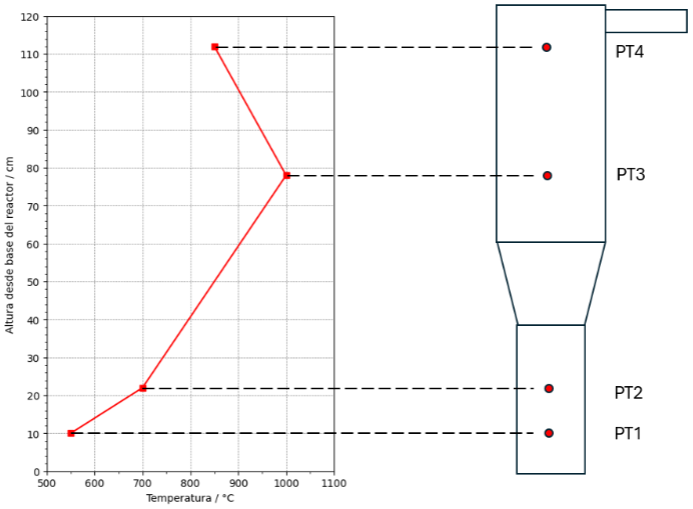
\includegraphics[width=0.6\linewidth]{figures/Caso1.png}
    \caption{Temperaturas alcanzadas al interior del reactor durante la pirólisis.}
    \label{Caso1}
\end{figure}

\subsection{Variables y parámetros}

En el ejercicio de reflexión desarrollado por el equipo de trabajo, se identificó y clasificó las siguientes variables y parámetros:

\begin{table}[h!]
\centering
\begin{tabular}{|l|l|lll}
\cline{1-2}
\textbf{Tipo} & \textbf{Variables}                                                                                        &  &  &  \\ \cline{1-2}
Dependiente   & \begin{tabular}[c]{@{}l@{}}Velocidad de la partícula ($V_p$), Velocidad del fluido ($V_f$) Coeficiente de convección ($h$),\\ Densidad del fluido ($\rho_f$),  Viscosidad cinemática ($\nu$), Número de Prandtl ($Pr$),\\ Número de Nusselt ($Nu$), Coeficiente de arrastre  ($C_d$), Temperatura del fluido, Temperatura de la partícula\end{tabular}                                                                                              &  &  &  \\ \cline{1-2}
Independiente & Tiempo (t), Posición vertical de la partícula                                                                                                                 &  &  &  \\ \cline{1-2}
Parámetro     & \begin{tabular}[c]{@{}l@{}}Diámetro de la partícula ($D$), Diámetro interno inferior y superior del reactor,\\ Altura del reactor, Coeficiente de arrastre $C_d$, Densidad del carbonizado,\\ Temperatura inicial del flujo, Flujo volumétrico del fluido, Masa de la partícula ($m_p$),\\ Área de sección transversal expuesta al fluido, Gravedad ($g$)\end{tabular} &  &  &  \\ \cline{1-2}
\end{tabular}
\end{table}


\subsection{Modelamiento matemático}

\subsubsection{Objetivo y alcance} 
El primer modelo que se realizó tiene como objetivo predecir la trayectoria (posición y velocidad) y la evolución en el tiempo de la temperatura de una partícula esférica carbonizada en el transcurso de su trayectoria vertical en un reactor de lecho fluidizado, en el que asciende a un flujo de nitrógeno a unas condiciones de operación determinadas experimentalmente. Éste modelo se fundamenta principalmente en la fuerza de arrastre ejercida por el gas y la transferencia de calor por convección.



El segundo modelo, supone ser el refinamiento del primer modelo pero teniendo en cuenta la radiación del sistema y los efectos de la flotación de la partícula. Su alcance deberá ser aún más preciso y completo que el primero para un experimento real. 

\subsubsection{Desarrollo matemático del modelo}
Iniciamos con el volumen de control en la propia partícula esférica de carbonizado, escogida por el equipo de trabajo debido al interés por conocer su trayectoria, velocidad y temperatura a lo largo del reactor. Sobre la partícula se tiene en cuenta la masa en dirección vertical descendente, y las fuerzas externas de arrastre ($F_d$) y la velocidad de flujo, en dirección vertical ascendente.

\begin{figure}[H]
    \centering
    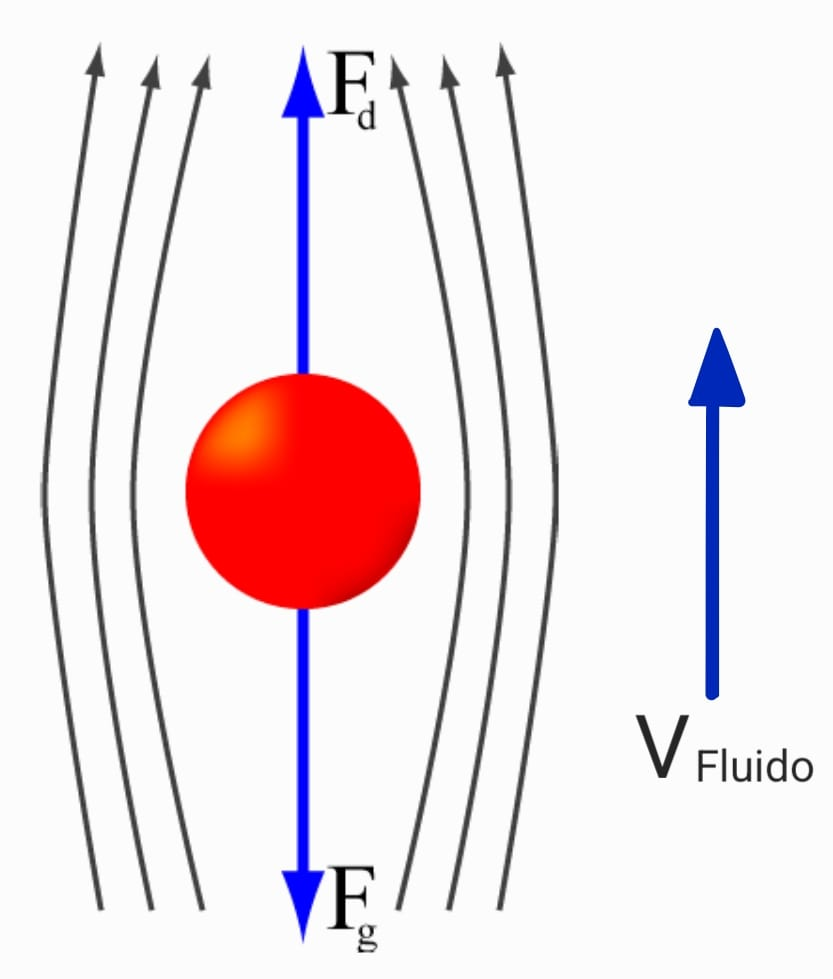
\includegraphics[width=0.2\linewidth]{Imagen de WhatsApp 2025-05-09 a las 11.36.50_4a59f02e.jpg}
    \caption{Diagrama de partícula}
    \label{Diagrama partícula}
\end{figure}

Con éste diagrama en mente, utilizamos la segunda ley de Newton en el eje z la cual nos plantea que,

\begin{equation}
    \sum_{}^{}F_{z}=ma
\end{equation}

por lo tanto,

\begin{equation}
    m_{p}\frac{dv}{dt}=F_{b}+F_{d}-F_{g}
    \label{Mov}
\end{equation}

donde $F_g$ representa el peso de la partícula, $F_b$ el empuje de flotación y $F_d$ es la fuerza de arrastre debida al fluido (la cual se asume con sentido hacia arriba ya que el gas asciende). Aquí como el modelo 1 al ser simplificado, se despreciará la fuerza de empuje $F_b$ y se reemplaza la fuerza de arrastre $F_d$ en su forma más genérica de tal modo que

\begin{equation}
    m_{p}\frac{dv}{dt}=\frac{1}{2}C_{d}\rho_f A v^{2}-m_{p}g
\end{equation}

donde $C_d$ es el coeficiente de arrastre, $m_p$ es la densidad de la partícula $\rho_p$ por unidad de volumen (considerando la geometría de la partícula idealmente como una esfera), $A$ es el área transversal de la partícula y $v$ la velocidad de la partícula respecto a la velocidad fluido(\cite{white2011fluid}).

\begin{equation}
    \rho_pV_p\frac{dv}{dt}=\frac{1}{2}C_{d}\rho_fA(v_{p}-v_{f})^{2}-g
    \label{4}
\end{equation}

Para continuar con éste desarrollo, se debe plantear primero la ecuación de continuidad para determinar la velocidad del fluido y consecuentemente, la velocidad de la partícula, por lo que en régimen estacionario y para un flujo unidireccional en $z$ el principio de conservación de masa en estado estacionario se escribe como:

\begin{equation}
    \dot{m}_{in}=\dot{m}_{out}
\end{equation}

es decir,
\[
    \rho_{in}v_{in}A_{in}=\rho_{out}v_{out}A_{out}
\]

Bajo las condiciones del nitrógeno en el enunciado del caso, se puede asumir que el fluido es incompresible o cuasi-incompresible por lo que se tomará $\rho\simeq $ constante, simplificando

\begin{equation}
    v_{in}A_{in}=v_{out}A_{out}=\dot{\forall}
\end{equation}

Donde se tiene que, para una altura cualquiera $z$ en el reactor, la velocidad local del gas de nitrógeno debe ajustarse para conservar el caudal volumétrico $\dot{\forall}$, ya que no existe acumulación de masa. Por lo tanto, la velocidad del fluido $v_f$ es:

\begin{equation}
    v(z)\cdot A(z)=\dot{\forall} \Rightarrow v_f(z)=\frac{\dot{\forall}}{A(z)}
    \label{Vel_f}
\end{equation}

Habiendo calculado la velocidad del fluido $v_f$, procedemos a calcular la velocidad de la partícula $v_p$ devolviéndonos a la ecuación \ref{4} nuevamente. En ésta, aún desconocemos el coeficiente de arrastre $C_p$, la cual se puede hallar a través de la ecuación de correlación de Schiller-Naumann, típica para esferas en flujo laminar/transicional la cual plantea:

\begin{equation}
    C_{d}=\frac{24}{Re}(1+0.15Re^{0.687})
    \label{Coefarras}
\end{equation}

Ésta ecuación depende del número de Reynolds local $Re$, la cual depende a su vez de la velocidad del fluido $V_f$, el diámetro conforme la sección transversal del reactor cambia $D$, y la viscosidad cinemática del fluido $\mu$. 

\begin{equation}
    Re=\frac{vD}{\nu}
    \label{Re}
\end{equation}

Los valores de la viscosidad cinemática del fluido $\mu$ se tomaron de la figura \ref{Tabla propiedades}, los cuales se interpolaron a partir de las temperaturas medidas en cada punto del reactor.

\begin{figure}[H]
    \centering
    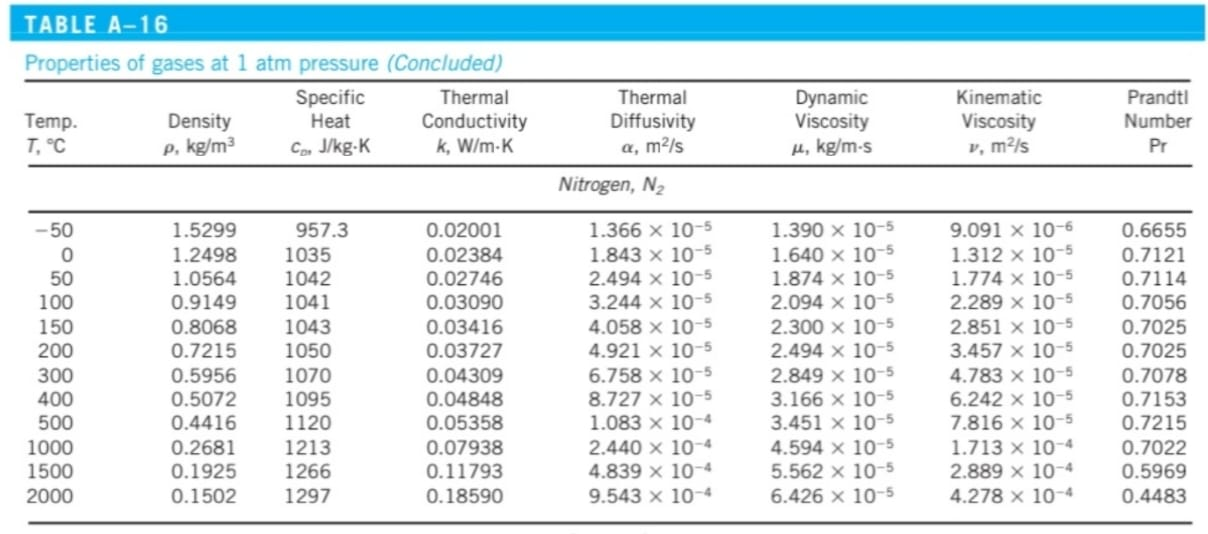
\includegraphics[width=0.7\linewidth]{figures/Imagen de WhatsApp 2025-05-10 a las 16.24.18_a4e1269a.jpg}
    \caption{Propiedades del gas de nitrógeno a presión de 1atm. Adaptado de \cite{cengel2013ebook}}
    \label{Tabla propiedades}
\end{figure}

Teniendo ésto en cuenta, se despeja la tasa de velocidad de la partícula respecto al tiempo y se resuelve ésta ecuación diferencial ordinaria de primer orden a través del método numérico \textit{Forward Euler}.
\begin{equation}
    \frac{dv}{dt}=\frac{3C_{d}\rho_{f}(v_{p}-v_{f})^{2}}{8\rho_{p}r}-g
\end{equation}

Con el fin de establecer un balance energía en este sistema abierto, se plantea la siguiente ecuación para este tipo de volúmenes de control (\cite{moran2010fundamentals}).

\begin{equation}
    \frac{dU}{dt}=\dot{Q}-\dot{W}
    \label{1Ley}
\end{equation}

El sistema no realiza ningún sistema mecánico por lo que $\dot{W}=0$, y el único mecanismo de transferencia de energía es convección térmica desde el gas de nitrógeno hacia la superficie de la partícula. Entonces, se procede a plantear la energía térmica $U$ y por la Ley de enfriamiento 
 de Newton $\dot{Q}_{convec}$.

\begin{equation}
    m_{p}C_{p}dT=hA(T_{\infty }-T)dt
\end{equation}

donde, 

\begin{itemize}
    \item $C_p$ es el calor específico de la partícula, el cual será de $1,52 kJ/kg.K$ (\cite{hornoRotatorio})
    \item $h$ es el coeficiente de convección.
    \item $A$ es el área superficial de la partícula.
    \item $T_{\infty }$ es la temperatura del fluido.
    \item $T$ es la temperatura de la partícula.
\end{itemize}

Como ecuación diferencial separable, se puede ordenar de la siguiente manera para resolverlo numéricamente posteriormente.

\begin{equation}
    m_{p}C_{p}\frac{dT}{dt}=hA(T_{\infty }-T)
    \label{convec}
\end{equation}

Para encontrar el coeficiente de convección $h$ se obtiene mediante la correlación de Nusselt para esfera en flujo forzado (Ranz–Marshall):

\begin{equation}
    Nu= 2+(0.4Re^{1/2}+0.06Re^{2/3})Pr^{0.4}, 
    \label{Nu}
\end{equation}

Para la cual ya tenemos el número de Reynolds $Re$ con la ecuación \ref{Re} y el número de Prandlt $Pr$ interpolando los valores de la figura \ref{Tabla propiedades} respecto a las temperaturas tomadas del experimento. Una vez tenemos los valores de $Nu$, procedemos a calcular $h$ con la siguiente ecuación:

\begin{equation}
    h=\frac{Nu \ k}{D}
    \label{h}
\end{equation}

donde $k$ es la conductividad térmica del gas del nitrógeno, con valores nuevamente obtenidos a través de las interpolaciones de la figura \ref{Tabla propiedades}. Así, nos queda la ecuación de la temperatura de la partícula en función del tiempo:

\begin{equation}
    \frac{dT_{p}}{dt}=\frac{hA(T_{\infty }-T)}{ m_{p}C_{p}}
\end{equation}


\subsection{Desarrollo Herramienta Computacional}

La función principal del código comienza cargando los parámetros del reactor y de la partícula (flujo volumétrico, geometría, radio, densidad, paso de tiempo, etc.), y crea vectores para almacenar posición, velocidad y temperatura inicial. Luego entra en un bucle temporal donde, en cada paso: calcula el área transversal según la altura, obtiene la velocidad del gas y la temperatura del fluido por interpolación, interpola las propiedades del gas (densidad, viscosidad, conductividad, Prandtl), evalúa el número de Reynolds y de ahí el coeficiente de arrastre. Después calcula las derivadas de velocidad (por arrastre y peso) y de temperatura (por convección), integra estas EDO con método explícito de Euler, actualiza posición, velocidad y temperatura de la partícula y almacena todos los resultados. Al finalizar el bucle (cuando la partícula sale del reactor o se alcanza el tiempo máximo), llama a plotter.py para generar las gráficas de posición, velocidad, temperatura y coeficientes en función del tiempo.

\begin{figure}[H]
    \centering
    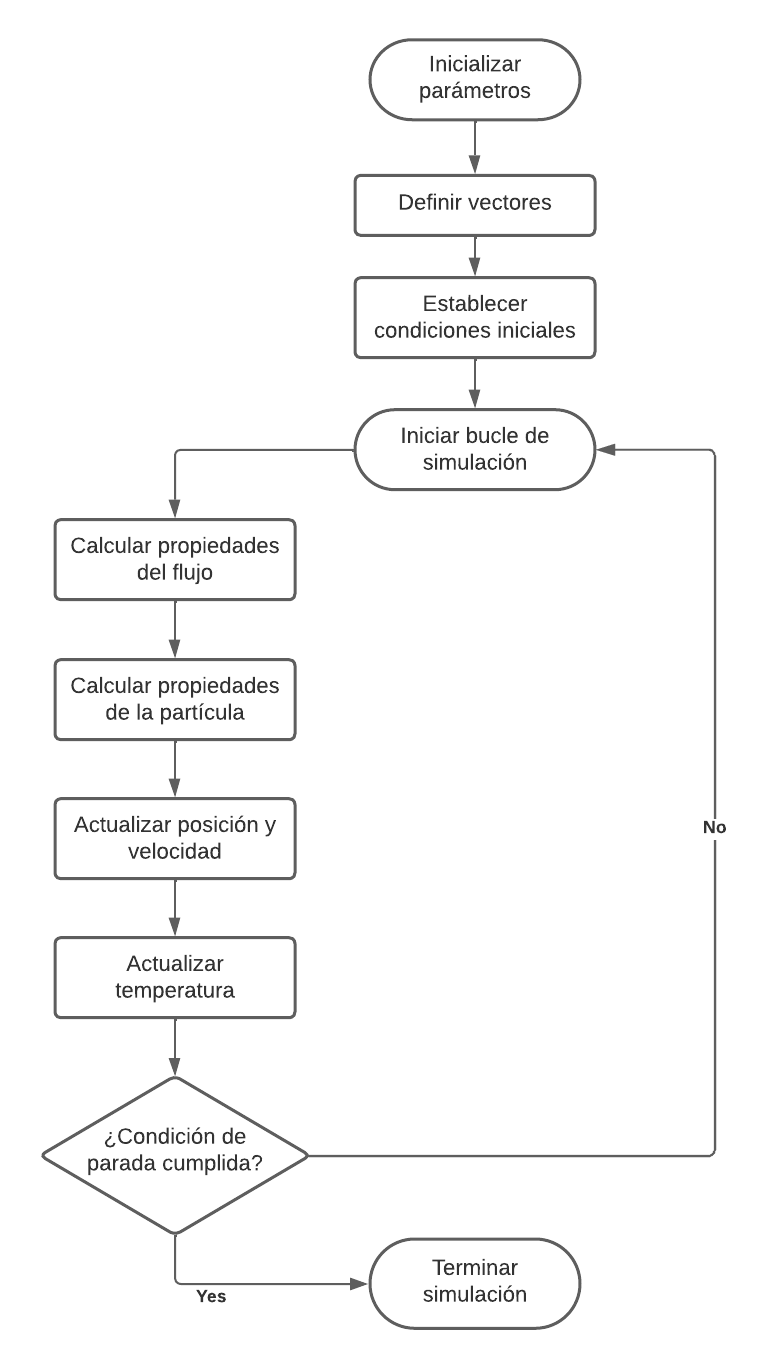
\includegraphics[width=0.45\linewidth]{figures/Blank diagram.png}
    \caption{Diagrama de flujo de la función principal del modelo 1.}
    \label{Diagrama de flujo}
\end{figure}

La función principal se apoya en otras funciones, las cuales llama en su código para funcionar. Por un lado, crossArea(z) determina el área transversal del reactor según la altura para obtener la velocidad local del gas; tempInterp(z) interpola linealmente la temperatura del gas a partir de datos experimentales; e interpolationMachine(T) interpola apartir de Rungr Kutta las propiedades del nitrógeno (densidad, viscosidad cinemática, conductividad y número de Prandtl) en función de esa temperatura. A partir de estas propiedades, dragCoeff(Re) calcula el coeficiente de arrastre con la correlación de Schiller–Naumann y hConvection(d,T,Re,Pr,k) evalúa el coeficiente de convección aplicando la corrección de Ranz–Marshall.

\begin{figure}[H]
    \centering
    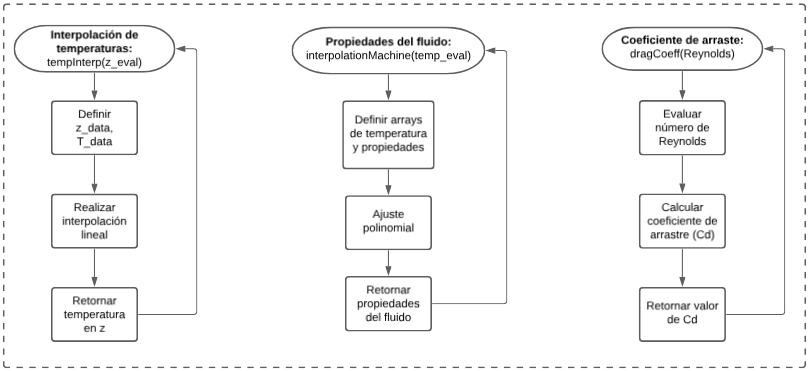
\includegraphics[width=0.85\linewidth]{figures/DiagramaAux.png}
    \caption{Diagrama de flujo de las funciones auxiliares del modelo 1.}
    \label{fig:enter-label}
\end{figure}

\subsection{Resultados obtenidos}
El modelo predice la evolución del comportamiento de la partícula a medida que asciende por el reactor. A continuación, se presentan los resultados obtenidos para el modelo simplificado, donde se mantuvieron constantes tanto la capacidad calorífica del carbonizado $C_p$ como el flujo volumétrico de entrada $\dot{\forall}$.

\begin{figure}[H]
    \centering
    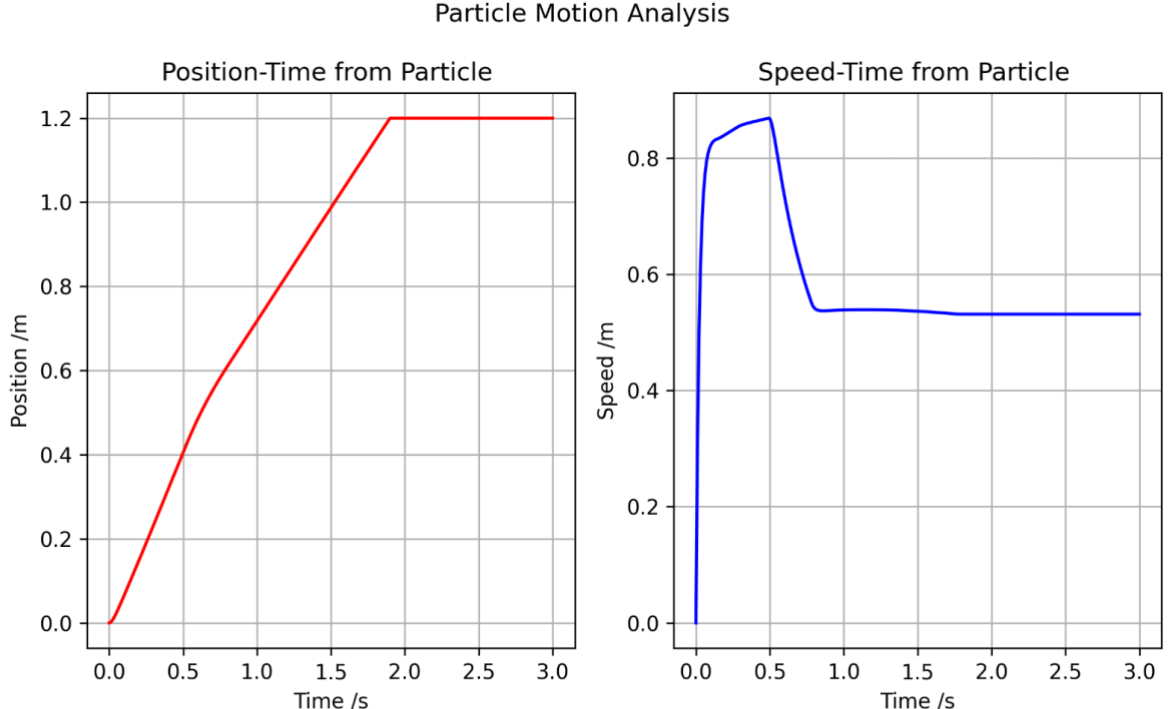
\includegraphics[width=0.6\linewidth]{figures/Cte4.png}
    \caption{Posición y velocidad de la partícula en función del tiempo.}
    \label{fig:enter-label}
\end{figure}

\begin{figure}[H]
    \centering
    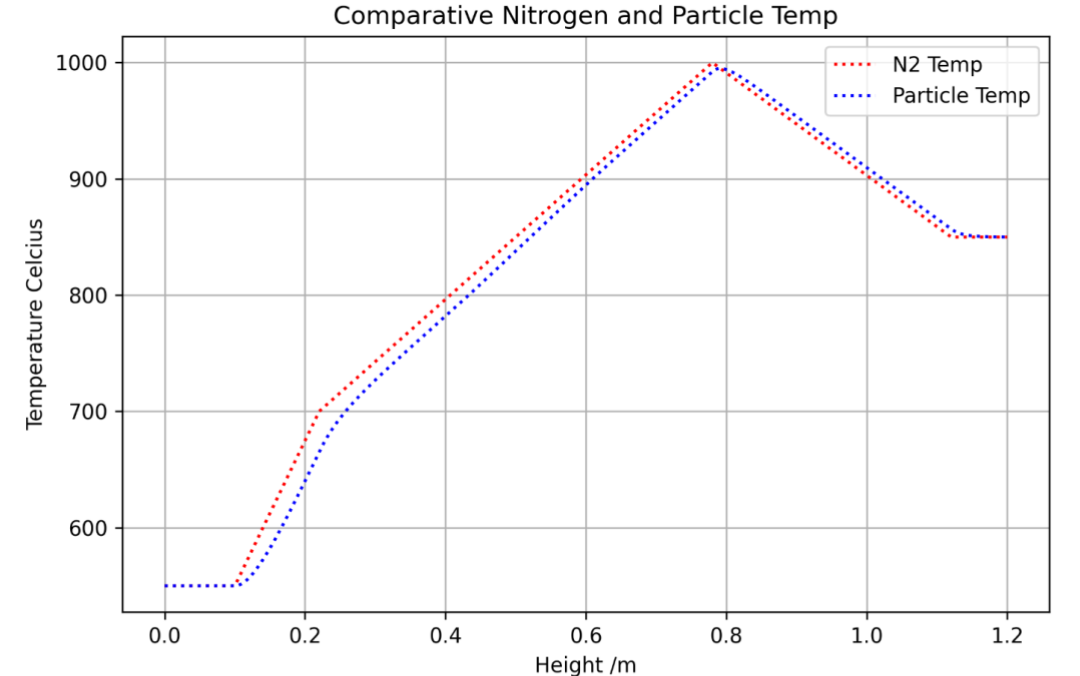
\includegraphics[width=0.5\linewidth]{figures/Cte1.png}
    \caption{Temperaturas del gas de nitrógeno y la partícula en función de la altura.}
    \label{fig:enter-label}
\end{figure}

\begin{figure}[H]
    \centering
    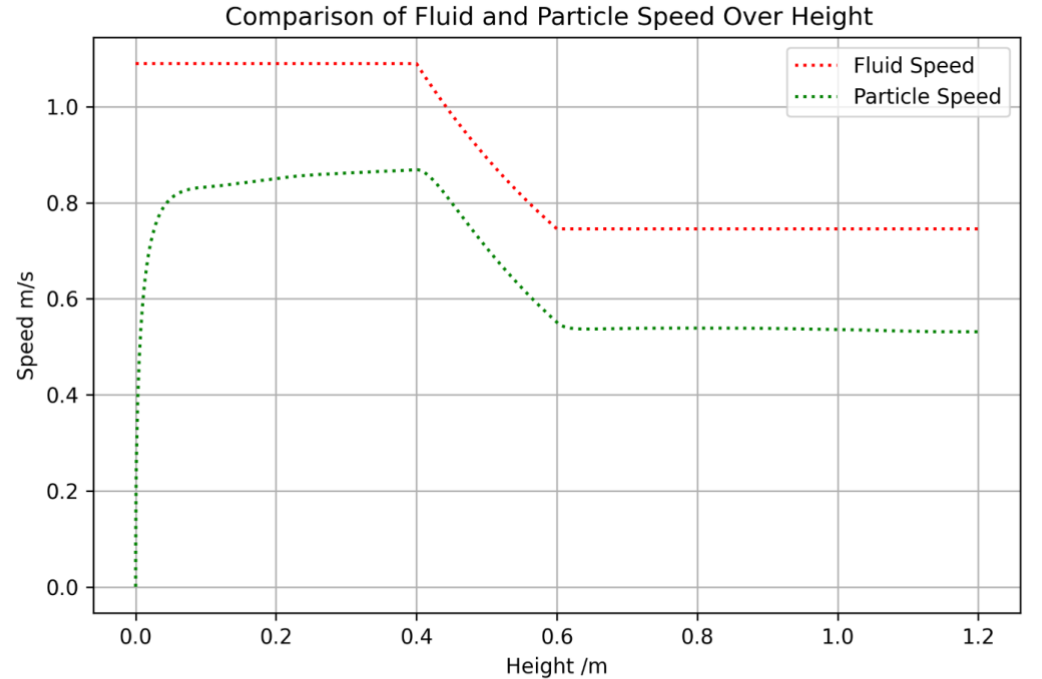
\includegraphics[width=0.5\linewidth]{figures/Cte2.png}
    \caption{Velocidad del gas de nitrógeno y la partícula en función de la altura.}
    \label{fig:enter-label}
\end{figure}

\begin{figure}[H]
    \centering
    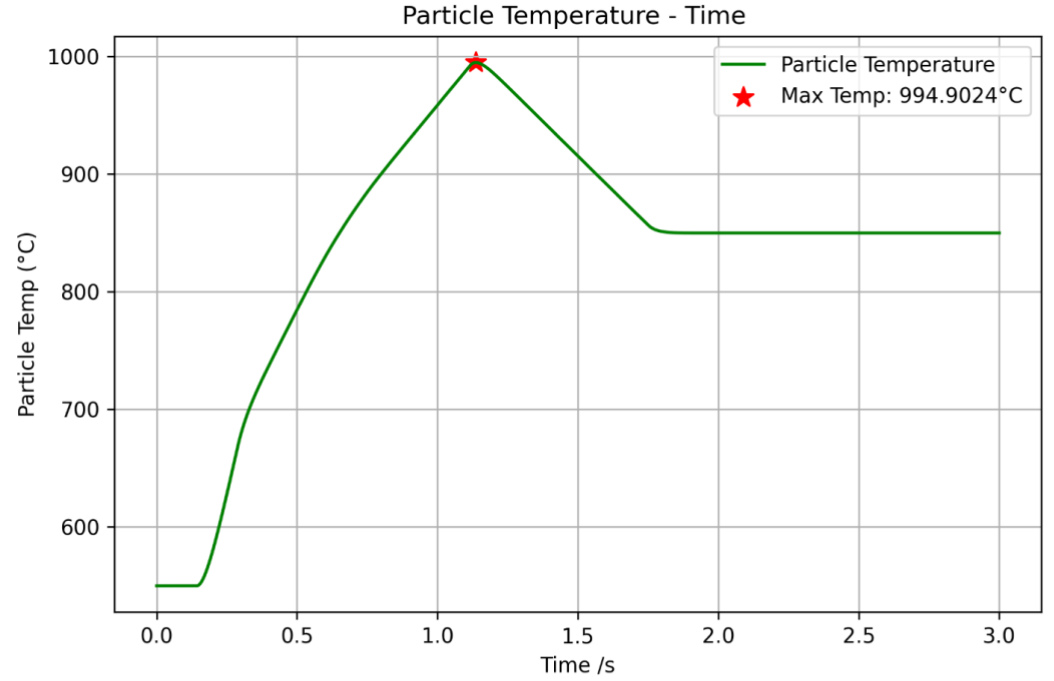
\includegraphics[width=0.5\linewidth]{figures/Cte5.png}
    \caption{Temperatura de la partícula en función del tiempo.}
    \label{fig:enter-label}
\end{figure}

\begin{figure}[H]
    \centering
    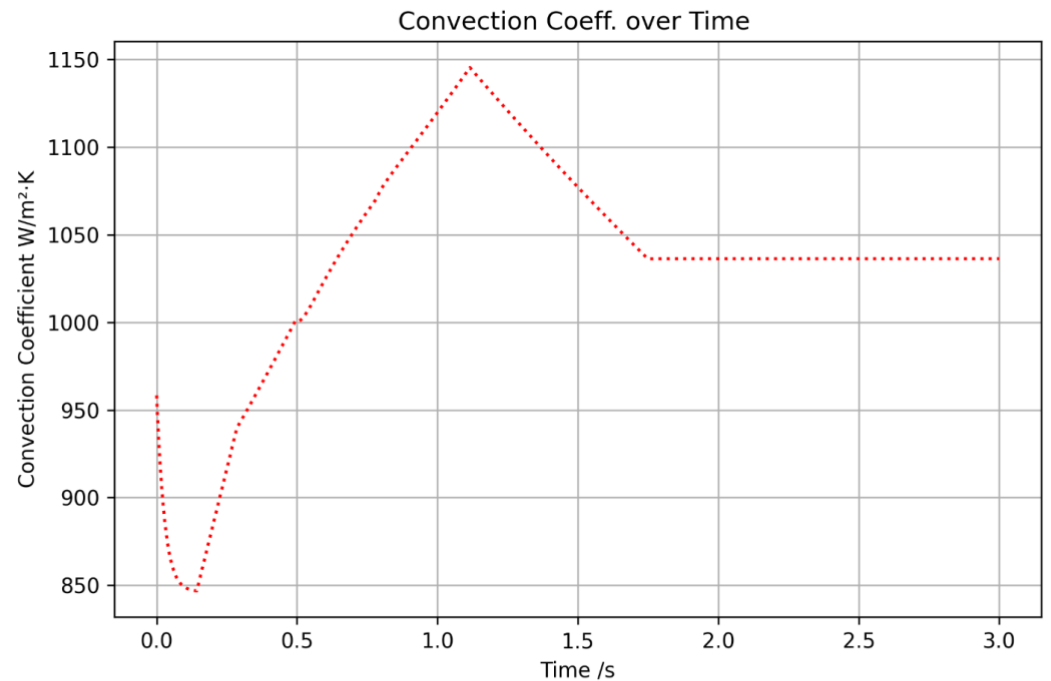
\includegraphics[width=0.5\linewidth]{figures/Cte6.png}
    \caption{Coeficiente de convección en función del tiempo.}
    \label{fig:enter-label}
\end{figure}

\begin{figure}[H]
    \centering
    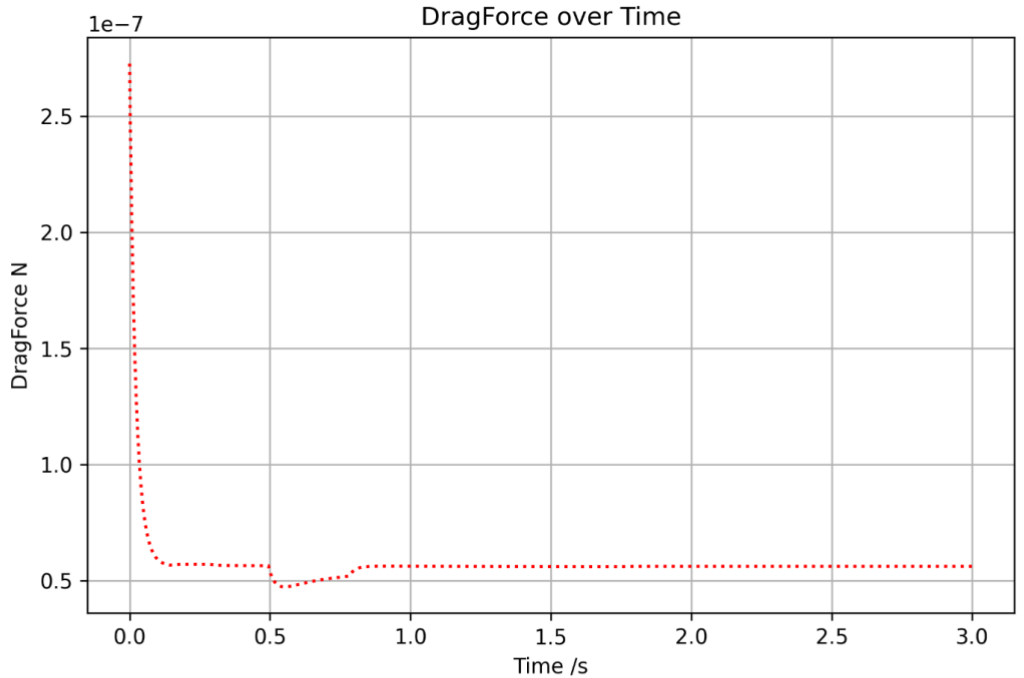
\includegraphics[width=0.5\linewidth]{figures/Cte7.png}
    \caption{Coeficiente de arrastre en función del tiempo.}
    \label{fig:enter-label}
\end{figure}


\subsection{Análisis de sensibilidad respecto a la capacidad calorífica del carbonizado $C_p$ y el flujo
volumétrico de entrada $\dot{\forall}$.}



\subsubsection{Efectos en la posición y velocidad de la partícula}

Se observa efectivamente que la variación del flujo volumétrico de entrada determina la velocidad del flujo como dicta la ecuación \ref{Vel_f} y, por ende, la fuerza de arrastre sobre la partícula. Como su relación es directamente proporcional, un mayor flujo volumétrico implica una velocidad del fluido más alta (número de Reynolds más grande), lo que ocasionará que la velocidad de la partícula tenderá a igualar la velocidad del fluido más rápido y así mismo, recorrer la distancia en el reactor más rápido. En cambio, a caudales bajos la velocidad del fluido es pequeña, el arrastre es débil y por éso la partícula avanza lentamente o no avanza.

\begin{figure}[H]
    \centering
    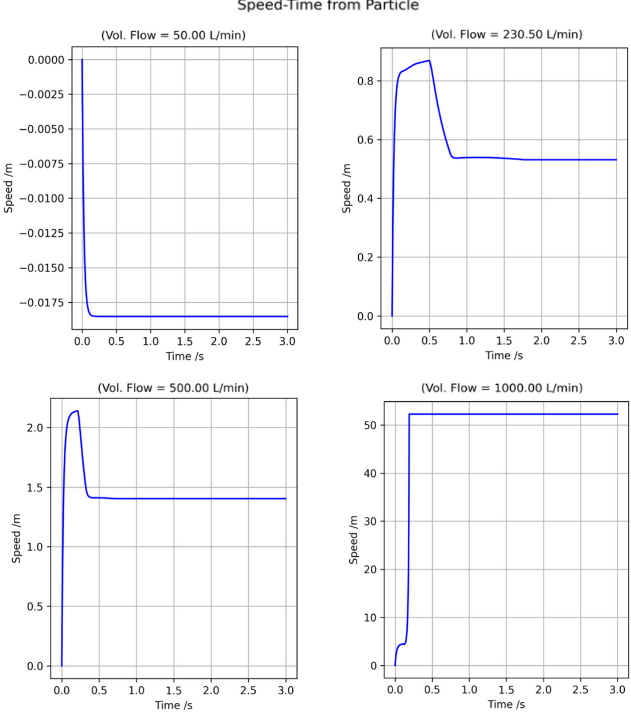
\includegraphics[width=0.6\linewidth]{figures/VelV.png}
    \caption{Gráficas de velocidad de la partícula en el tiempo, con distintos flujos volumétricos de entrada.}
    \label{fig:enter-label}
\end{figure}

En la gráfica de flujo volumétrico $\dot{\forall}=50 L/min$, la velocidad decrece debido a que la velocidad del fluido es tan baja que la fuerza de arrastre no logra vencer el peso de la partícula, por lo que ésta no puede ascender sino que desciende por acción de la gravedad. Sin embargo, si físicamente la partícula no puede descender en el reactor (no se determinó en el código), su posición y velocidad serían igual a cero.\\

En cuanto a la capacidad calorífica $C_p$ de la partícula, ésta no afecta significativamente en su posición y velocidad ya que éstas dependen en mayor medida del flujo volumétrico y del coeficiente de arrastre.


\subsubsection{Efectos en la temperatura de la partícula}

La variación de la capacidad calorífica $C_p$ demostró la relación inversamente proporcional con la temperatura de la partícula como se plantea matemáticamente en la ecuación \ref{convec}, pues entre más bajo fue la capacidad calorífica, la partícula alcanzó temperaturas más altas en menor tiempo para un mismo coeficiente convectivo $h$. En cambio para un $C_p$ mayor, la temperatura máxima fue menor y alcanzada en más tiempo por milisegundos.\\

Respecto al flujo volumétrico, se observó que la temperatura máxima se alcanzaba en menor tiempo cuando se elevaban los valores del flujo, debido a que la velocidad del flujo afecta directamente al coeficiente de convección $h$, por lo que a flujos altos, la partícula se calienta mucho más en un mismo intervalo de tiempo que a flujos bajos.\\

\begin{figure}[H]
    \centering
    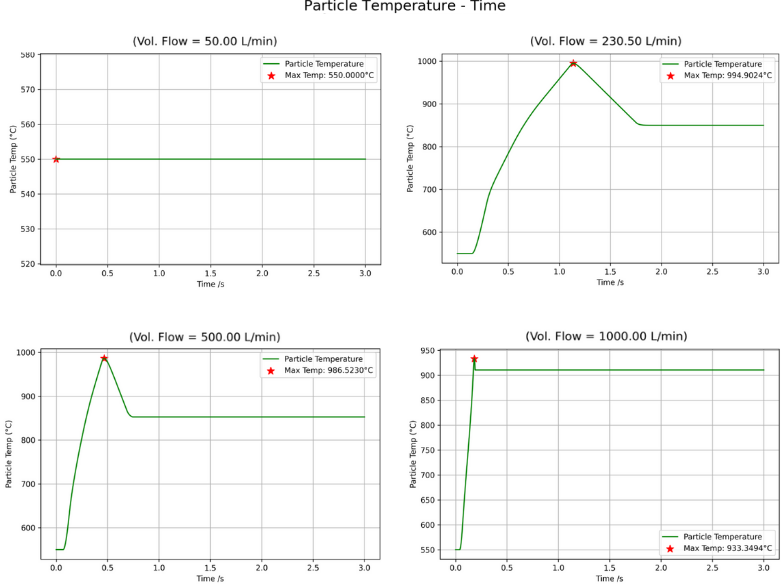
\includegraphics[width=0.7\linewidth]{figures/Temp1.png}
    \caption{Gráficas de temperatura de la partícula en el tiempo, con distintos flujos volumétricos de entrada.}
    \label{fig:enter-label}
\end{figure}

De nuevo, en un flujo tan bajo como $\dot{\forall}=50 L/min$ la posición y la velocidad de la partícula tienden a decrecer, por tanto, la temperatura de ésta no aumentará más de los $550 \degree C$ (su temperatura de entrada).

\subsubsection{Comportamiento del coeficiente de convección \texorpdfstring{$h$}{h}}

Se evidencia en los resultados que el coeficiente de convección $h$ aumenta con la velocidad del flujo del fluido $V_f$, siendo coherente con la ecuación \ref{h} donde se demuestra la dependencia directa del coeficiente de convección $h$ con la conductividad térmica del fluido $k$, y el número de Nusselt que depende a su vez del número de Reynolds. Por lo tanto, al aumentar el caudal del gas de nitrógeno, el flujo pasará de uno laminar a uno turbulento, lo que resultará en el incremento del coeficiente de convección $h$ como se muestra en la siguiente imágen.

\begin{figure}[H]
    \centering
    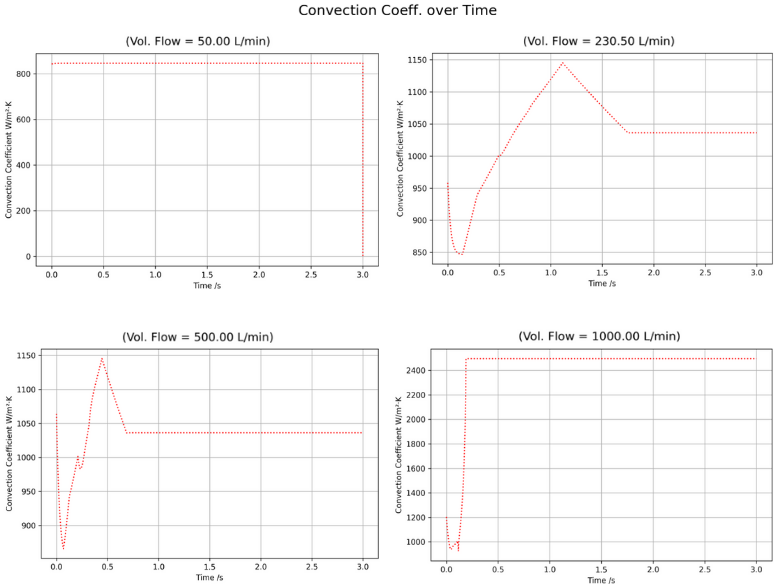
\includegraphics[width=0.7\linewidth]{figures/Convec1.png}
    \caption{Gráficas del coeficiente convectivo en el tiempo, con distintos flujos volumétricos de entrada.}
    \label{fig:enter-label}
\end{figure}

La capacidad calorífica $C_p$ en el caso contrario no influyó en el coeficiente de convección $h$, ya que éste está más relacionado al estado del fluido y no al calor específico de la partícula. 

\subsubsection{Comportamiento del coeficiente de arrastre $C_d$}

El coeficiente de arrastre $C_d$ al estar estrechamente relacionado con el número de Reynolds $Re$ (como se expresa en la ecuación \ref{Coefarras}) depende del flujo volumétrico del fluido $\forall$. Se observa que a bajos flujos el coeficiente de arrastre $C_d$ es elevado y casi constante, mientras que al aumentar el flujo el $C_d$ cae estabilizándose conforme la partícula alcanza velocidad cercana a la del fluido. En cuanto a la capacidad calorífica $C_p$ no se percibió mayor cambio respecto al coeficiente de arrastre $C_p$.

\begin{figure}[H]
    \centering
    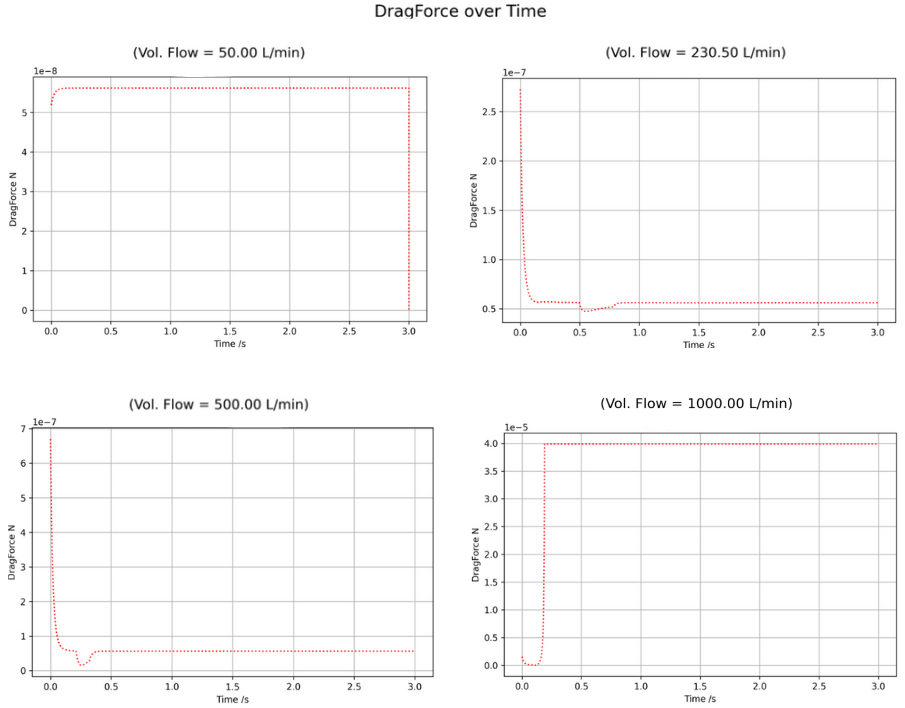
\includegraphics[width=0.7\linewidth]{figures/Coefarras1.png}
    \caption{Gráficas del coeficiente de arrastre de la partícula en el tiempo, con distintos flujos volumétricos de entrada.}
    \label{fig:enter-label}
\end{figure}

\subsection{Conclusiones del modelo simplificado}

El flujo volumétrico del fluido demostró ser la variable dominante en éste modelo convectivo simplificado. Su aumento incrementa la velocidad del fluido y por ende, el número de Reynolds, lo que eleva tanto el coeficiente convectivo $h$ como la fuerza de arrastre $C_d$ experimentada. En consecuencia, con flujos altos la partícula se traslada más rápido (en posición y velocidad) y se calienta mucho más rápido debido al mayor coeficiente de convección $h$.\\

En cambio, la capacidad calorífica $C_p$ afecta principalmente la respuesta térmica, pues a menores valores de $C_p$ se produce un calentamiento más rápido, y viceversa como ya se explicó. Por ello, los efectos predominantes desde el punto de vista dinámico, es la magnitud del flujo volumétrico $\forall$ que controla la trayectoria y velocidad, y desde el punto de vista térmico, la capacidad calórica de la partícula $C_p$ y el propio flujo (que modifica el $h$) actúan de modo conjunto. En resumen, en flujos más altos de fluido, la partícula se mueve más rápido y su transferencia de calor será también elevada. Sin embargo, si la capacidad calorífica de la partícula es alta, su temperatura aumentará lentamente, y si es 
baja alcanzará rápidamente la temperatura del fluido. Éste comportamiento es consistente con lo que predicen las ecuaciones y correlaciones físicas utilizadas para modelar la convección y el arrastre de éste experimento.

\subsection{Refinamiento del modelo}
En la segunda versión del modelo, se agregan dos efectos adicionales: radiación térmica y flotación (empuje de Arquímedes), los cuales se reflejarán en nuevas ecuaciones de movimiento y energía que darán como resultado un modelo más preciso del experimento.\\

Retomando desde la ecuación \ref{Mov} en la cual ahora si tenemos en cuenta las fuerzas de flotación $F_du$, se desarrolla la sumatoria de fuerzas en sus expresiones más generales:

\begin{equation}
    m_{p}\frac{dv}{dt}=\rho_{f}V_{p}g +\frac{1}{2}C_{d}\rho_f A (v_{p}-v_{f})^{2}-m_{p}g
\end{equation}

Resultando la ecuación diferencial ordinaria para la velocidad de la partícula respecto al tiempo de la siguiente manera:

\begin{equation}
    \frac{dv}{dt}=g(\frac{\rho_{f}V_{p}}{m_{p}})+\frac{1}{m_{p}}(\frac{1}{2}C_{d}\rho_f A (v_{p}-v_{f})^{2})
\end{equation}

Dado que $\frac{\rho_{p}V_{p}}{m_{b}}=\frac{\rho_{f}}{\rho_{p}}$ el término de flotación modifica el valor de la gravedad.

Continuando con el balance de energía para éste modelo, nos adelantamos a la ecuación \ref{1Ley} para plantear no sólo el mecanismo de transferencia de energía por convección a través de la Ley de enfriamiento de Newton sino por radiación a través de la Ley de Stefan–Boltzmann, teniendo en cuenta nuevamente que el sistema no realiza ningún trabajo por lo que $\dot{W}=0$.

\begin{equation}
    \frac{dU}{dt}=\dot{Q}_{convec}+\dot{Q}_{rad}
\end{equation}

\[
    m_{p}C_{p}\frac{dT_{p}}{dt}=hA(T_{\infty }-T_{p})+\varepsilon\sigma A(T_{\infty }^{4}-T_{p}^{4})
\]

Donde $\varepsilon$ es la emisividad de la superficie con el valor de 0.89 (tomado de \cite{etde_20278019}), $\sigma$ es la constante de Stefan-Boltzmann, $T_{\infty}$ la temperatura local del fluido, y $T_{p}$ la temperatura de la partícula. Reutilizando las ecuaciones para hallar el número de Reynolds \ref{Re}, el número de Nusselt \ref{Nu} y con ellas el coeficiente de convección \ref{h}, se despeja la ecuación diferencial para hallar la temperatura de la partícula en función del tiempo, nos queda:

\begin{equation}
    \frac{dT_{p}}{dt}=\frac{hA(T_{\infty }-T_{p})}{m_{p}C_{p}}+\frac{\varepsilon\sigma A(T_{\infty }^{4}-T^{4})}{m_{p}C_{p}}
\end{equation}

\subsection{Resultados obtenidos}

A continuación, se presentan los resultados obtenidos para el modelo refinado, donde se mantuvieron constantes tanto la capacidad calorífica del carbonizado $C_p$ como el flujo volumétrico de entrada $\dot{\forall}$.

\begin{figure}[H]
    \centering
    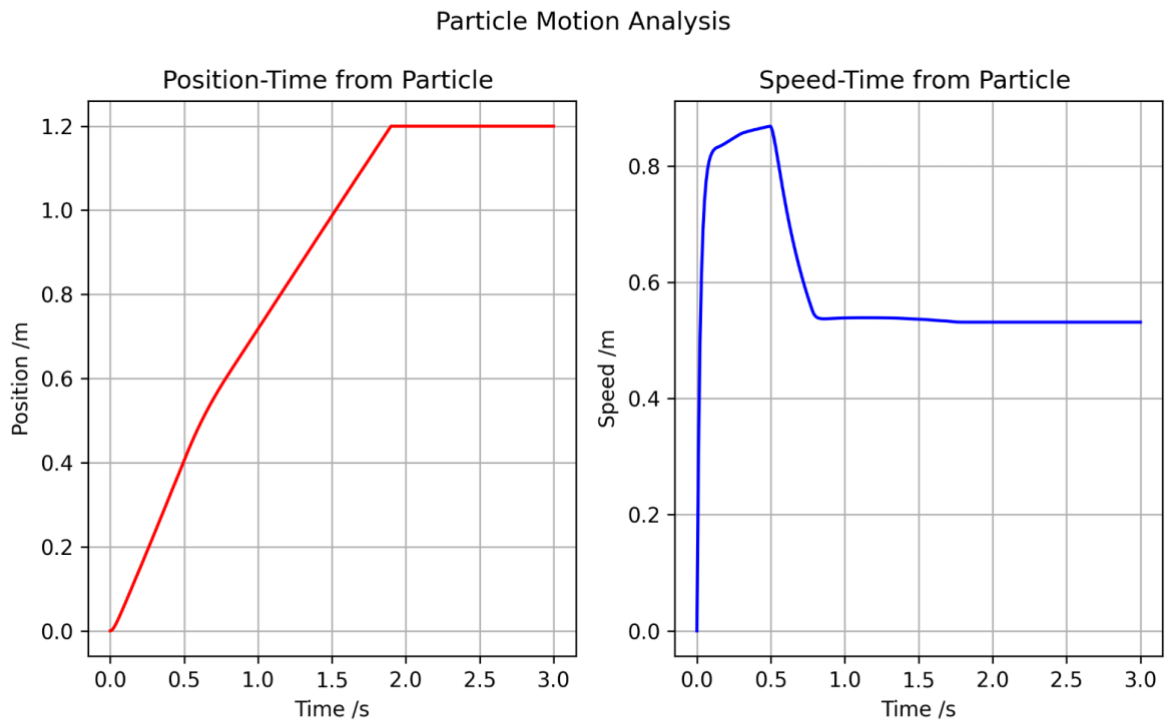
\includegraphics[width=0.6\linewidth]{figures/Rad1.png}
    \caption{Posición y velocidad de la partícula en función del tiempo.}
    \label{fig:enter-label}
\end{figure}

\begin{figure}[H]
    \centering
    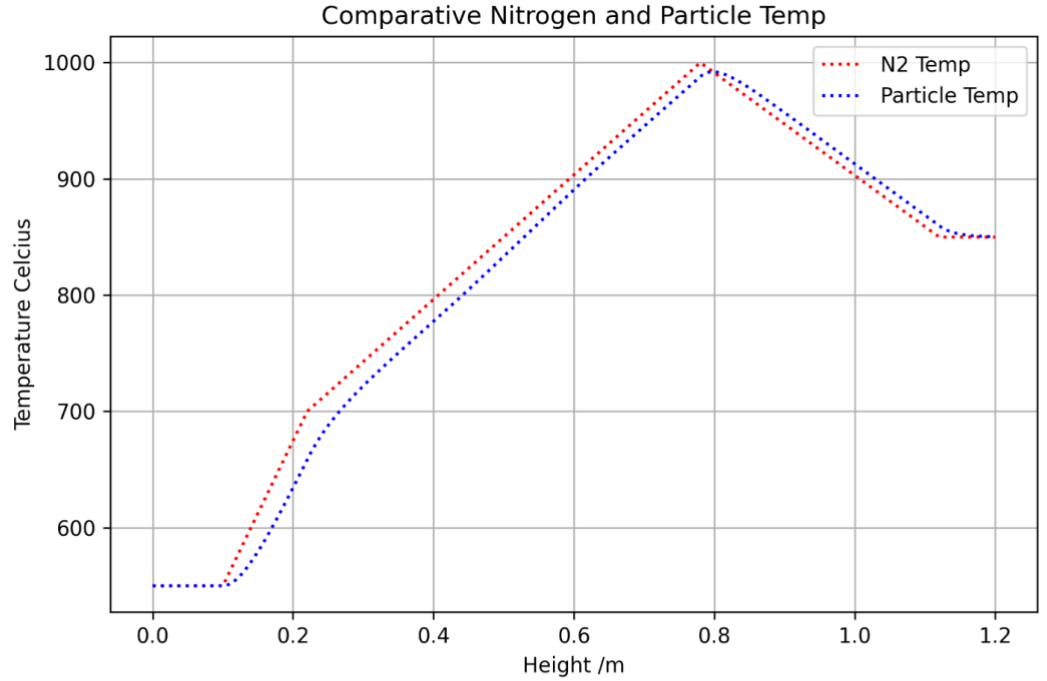
\includegraphics[width=0.5\linewidth]{figures/Rad2.png}
    \caption{Temperaturas del gas de nitrógeno y la partícula en función de la altura.}
    \label{fig:enter-label}
\end{figure}

\begin{figure}[H]
    \centering
    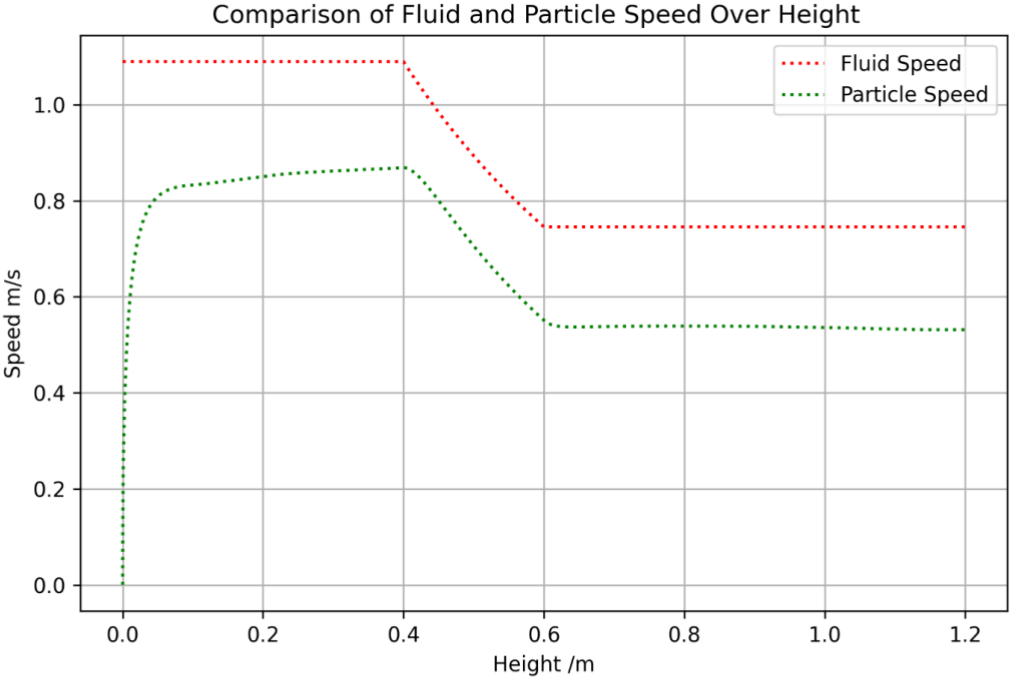
\includegraphics[width=0.5\linewidth]{figures/Rad3.png}
    \caption{Velocidad del gas de nitrógeno y la partícula en función de la altura.}
    \label{fig:enter-label}
\end{figure}

\begin{figure}[H]
    \centering
    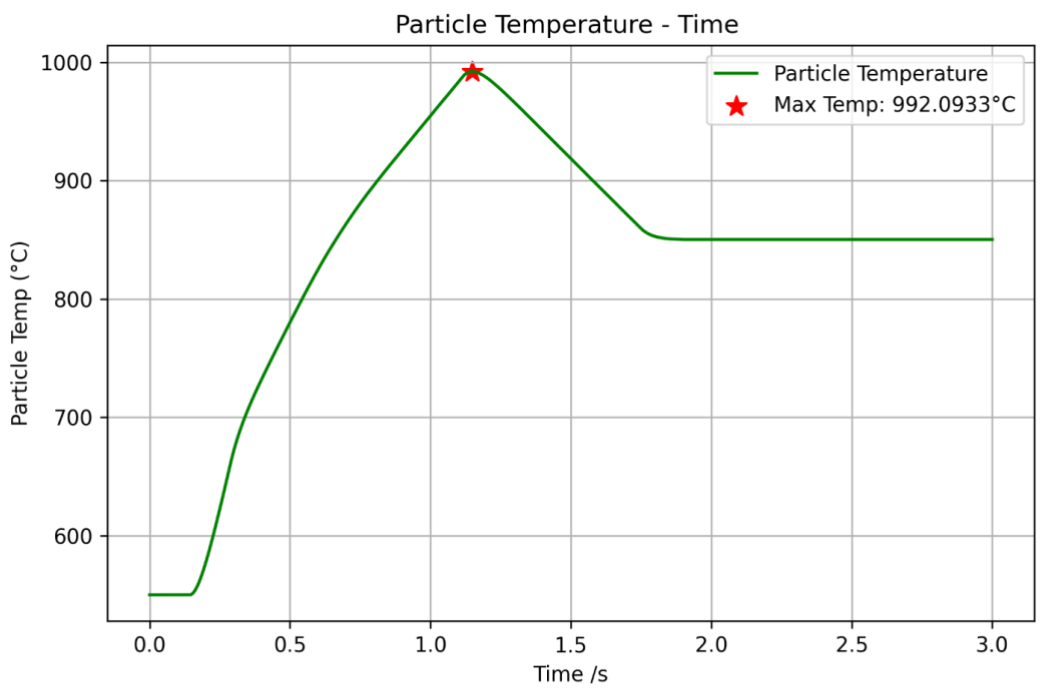
\includegraphics[width=0.5\linewidth]{figures/Rad4.png}
    \caption{Temperatura de la partícula en función del tiempo.}
    \label{fig:enter-label}
\end{figure}

\begin{figure}[H]
    \centering
    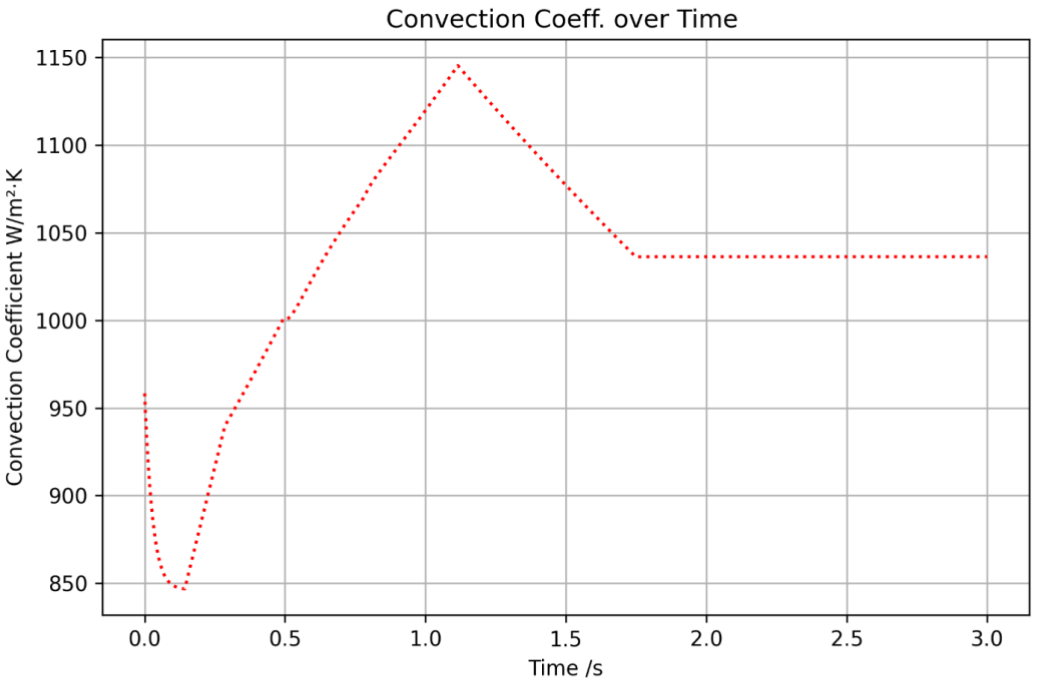
\includegraphics[width=0.5\linewidth]{figures/Rad5.png}
    \caption{Coeficiente de convección en función del tiempo.}
    \label{fig:enter-label}
\end{figure}

\begin{figure}[H]
    \centering
    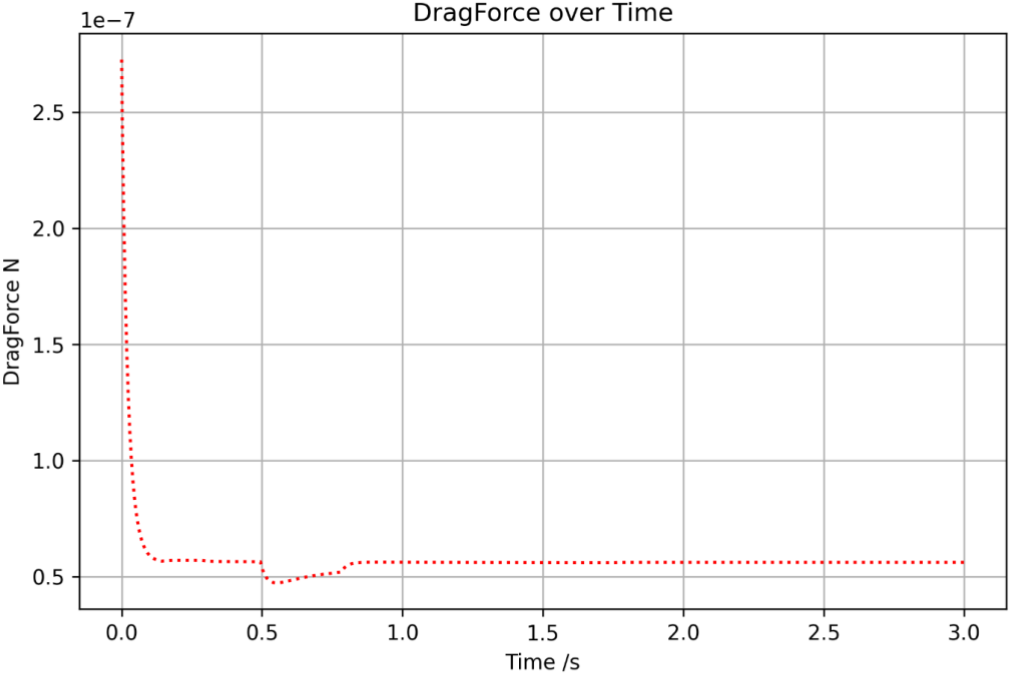
\includegraphics[width=0.5\linewidth]{figures/Rad6.png}
    \caption{Coeficiente de arrastre en función del tiempo.}
    \label{fig:enter-label}
\end{figure}

\subsection{Análisis de sensibilidad respecto a la capacidad calorífica del carbonizado $C_p$ y el flujo
volumétrico de entrada $\dot{\forall}$.}

\subsubsection{Efectos en la posición y velocidad de la partícula}

Al crecer el flujo volumétrico aumenta la velocidad del fluido, lo que incrementa drásticamente la fuerza de arrastre $F_d$  y, por tanto, en valores más altos en velocidad y desplazamiento. Por otro lado respecto a la capacidad calorífica, un $C_p$ alto significa que la partícula se calienta lentamente para igualar la temperatura del fluido mientras que un $C_p$ bajo da lugar a un calentamiento rápido, y ésto reduce la fuerza de flotación al depender de la densidad del fluido.

\begin{figure}[H]
    \centering
    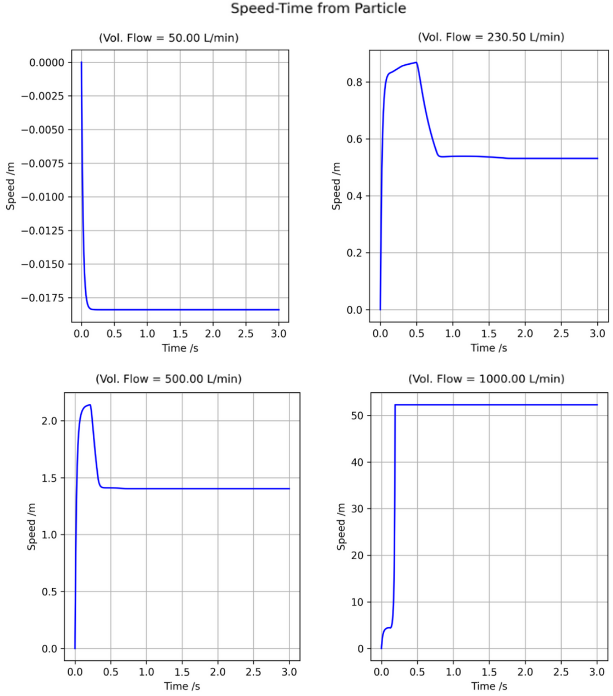
\includegraphics[width=0.6\linewidth]{figures/Radcte.png}
    \caption{Graficas de la velocidad de la partícula en función del tiempo, con distintos flujos volumétricos. Modelo refinado.}
    \label{fig:enter-label}
\end{figure}

En resumen, un flujo volumétrico alto impulsa a la partícula a moverse más rápido y a recorrer una distancia mayor, y al aumentar su temperatura, se favorece el ascenso de la partícula por efecto de la flotación. Por su parte, un $C_p$ alto modera estos efectos, ya que ralentiza el calentamiento de la partícula 

\subsubsection{Efectos en la temperatura de la partícula}

En los resultados se observa que un $C_p$ más alto significa que la partícula necesita más energía para calentarse, por lo que su temperatura aumenta más lentamente frente al mismo aporte de calor. Por otro lado, un flujo volumétrico más alto incrementa el coeficiente de convección ($h$) y, por ende, el intercambio de calor con el fluido, además la radiación introduce un aporte constante de calor, que eleva gradualmente la temperatura de la partícula y del fluido. En conjunto, un $C_p$ alto atenúa los cambios de temperatura (menor tasa de calentamiento), mientras que un flujo alto y mayor radiación provoca variaciones más rápidas en la temperatura.

\begin{figure}[H]
    \centering
    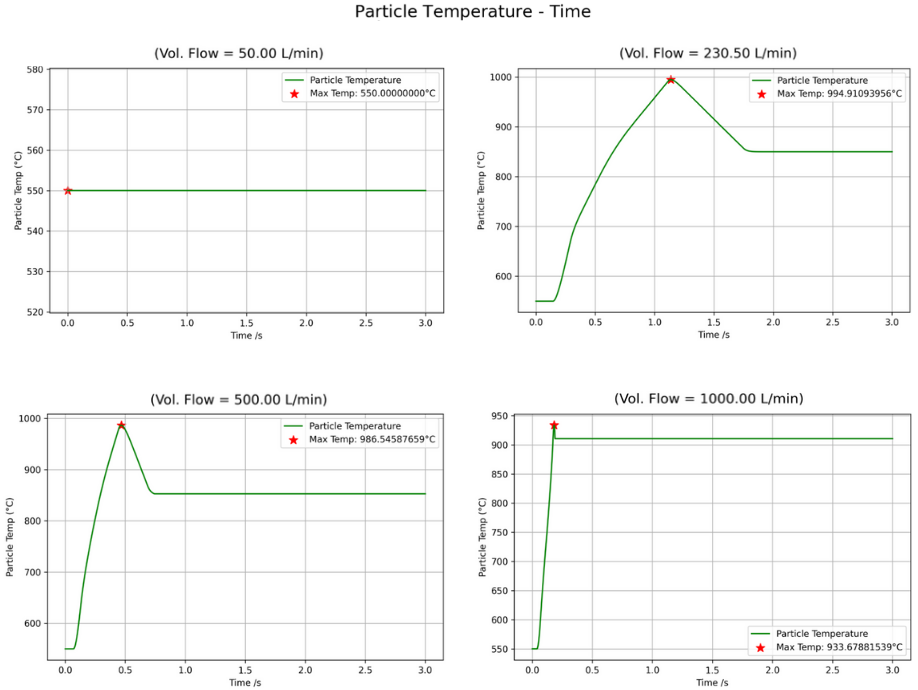
\includegraphics[width=0.7\linewidth]{figures/Radcte2.png}
    \caption{Graficas de la temperatura de la partícula en función del tiempo, con distintos flujos volumétricos. Modelo refinado.}
    \label{fig:enter-label}
\end{figure}

\subsubsection{Comportamiento del coeficiente de convección $h$}

En los resultados se puede apreciar cómo el coeficiente de convección ($h$) varía principalmente con el flujo de entrada. En condiciones de flujo laminar, $h$ tiende a ser bajo. Sin embargo, al aumentar el caudal volumétrico, el flujo se vuelve más turbulento lo que mejora el contacto entre el fluido y la superficie de la partícula. Esto facilita que el calor se transfiera más rápido, elevando significativamente el valor de $h$.

\begin{figure}[H]
    \centering
    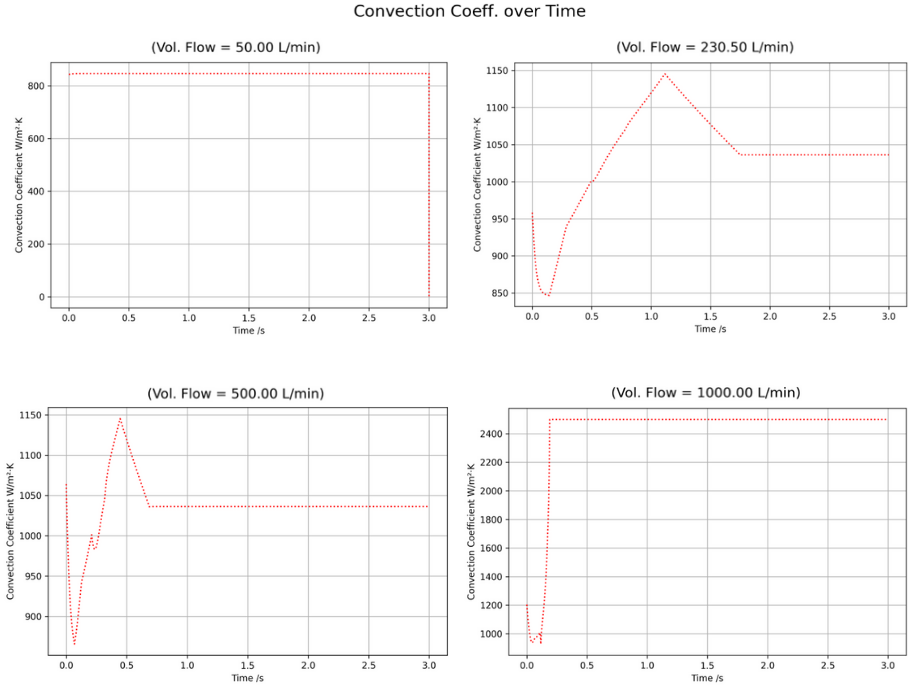
\includegraphics[width=0.7\linewidth]{figures/Radcte3.png}
    \caption{Graficas del coeficiente convectivo en función del tiempo, con distintos flujos volumétricos. Modelo refinado}
    \label{fig:enter-label}
\end{figure}

La capacidad calorífica ($C_p$) de la partícula no influye directamente en $h$ ya que éste está determinado sobre todo por la velocidad del fluido, su viscosidad y el tipo de flujo. La radiación por otro lado, cuando el flujo es alto, la diferencia de temperatura aumenta más la transferencia de calor, lo que también se refleja en valores más altos de $h$ en las gráficas.

\subsubsection{Comportamiento del coeficiente de arrastre $C_p$}

El coeficiente de arrastre $C_d$ depende directamente del número de Reynolds, y de la velocidad de la partícula respecto a la del fluido, por lo que el aumento del flujo volumétrico, aumenta la velocidad del fluido y el número de Reynolds lo que resulta en una disminución del $C_d$ según la correlación de Schiller–Naumann. Sin embargo, la fuerza de arrastre al depender también de la velocidad de la partícula y del flujo, el arrastre crece a mayor flujo incluso si $C_d$ disminuye. En cuanto a la capacidad calorífica $C_p$, su efecto sobre $C_d$ es indirecto y muy leve.

\begin{figure}[H]
    \centering
    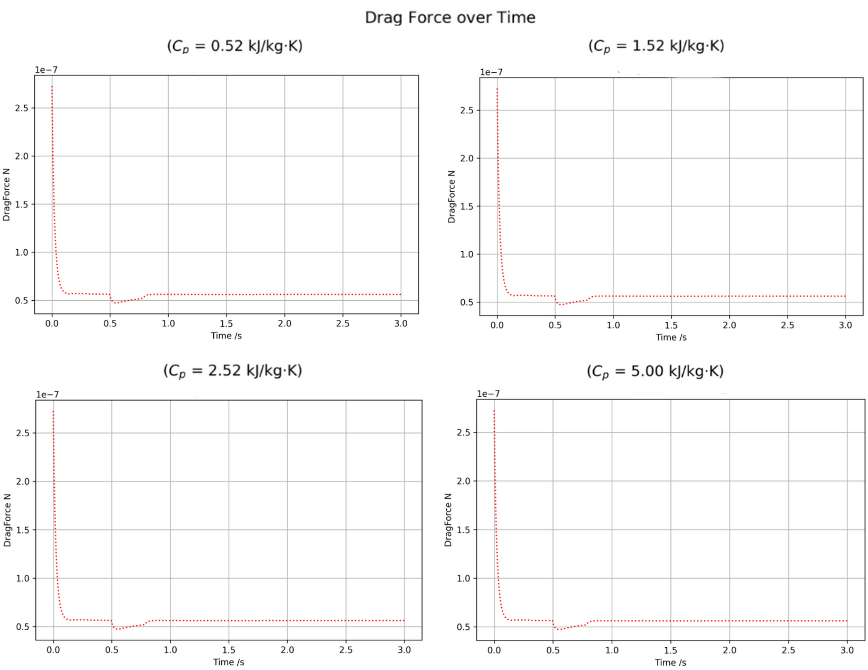
\includegraphics[width=0.7\linewidth]{figures/Radcte4.png}
    \caption{Graficas del coeficiente de arrastre en función del tiempo, con distintos flujos volumétricos. Modelo refinado}
    \label{fig:enter-label}
\end{figure}

\subsection{Conclusión de la comparativa entre el modelo simplificado y el refinado}

En el modelo refinado, la inclusión de la radiación y el empuje de flotación introduce dos mecanismos que aunque no alteran drásticamente la trayectoria básica de la partícula, sí modifican de forma notable su calentamiento y su aceleración neta. El modelo simplificado, en el que sólo se tiene en cuenta la convección, subestima la temperatura máxima de la partícula y omite el ligero impulso extra que aporta la flotación, por lo que predice una velocidad de ascenso y un grado de calentamiento menos realistas en condiciones extremas de flujo y temperatura. En cambio, el modelo refinado tiene en cuenta adicionalmente, la transferencia de calor por radiación, el cual eleva aún más la temperatura máxima en flujos altos, y el ligero empuje ascendente debido a la disminución de densidad del fluido, reflejando un calentamiento más acelerado y una velocidad más alta. Por lo tanto, mientras el modelo simplificado resulta ser suficiente para estimaciones preliminares, el modelo refinado ofrece una descripción más completa y precisa de la transferencia de calor y la dinámica de la partícula en un reactor real.


\section{Caso 2. Modelo para estudiar separación de vehículos de carga - 40\%}



\subsection{Contextualización del caso y su obejtivo}

El caso presentado se centra en el estudio de la separación entre vehículos de carga en una caravana automatizada, conocida como "micro-pelotón". Este tipo de configuración busca optimizar la distancia entre vehículos (denominada \textit{headway}) para minimizar la resistencia aerodinámica y, por ende, el consumo de combustible, mientras se garantiza una separación mínima que evite colisiones.

\begin{figure}[H]
    \centering
    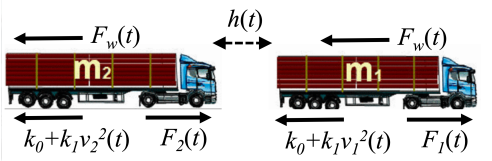
\includegraphics[width=0.75\linewidth]{Contexto 2do punto.png}
\end{figure}

\subsection{Estudio del Caso}

\subsubsection{Parametros y Variables}

Durante el ejercicio de reflexión llevado a cabo por el equipo de trabajo, se identificaron y clasificaron las siguientes variables y parámetros:

\begin{table}[h!]
\centering
\begin{tabular}{|l|l|lll}
\cline{1-2}
\textbf{Tipo} & \textbf{Variables}                                                                                        &  &  &  \\ \cline{1-2}
Dependiente   & \begin{tabular}[c]{@{}l@{}}Velocidad cada vehículo (\(v_i\)), Posición de cada Vehículo (\(x_i\)), Distancia de separación (\(h_i\)), \\ Consumo de Combustible, Consumo de potencia.\end{tabular}                                                                                              &  &  &  \\ \cline{1-2}
Independiente & Tiempo (t).                                                                                                                 &  &  &  \\ \cline{1-2}
Parámetro     & \begin{tabular}[c]{@{}l@{}}Fuerza propulsiva, Fuerza resistiva, Fuerza aleatoria del viento (Oscilante o pulsante)\\ Masa de los camiones, Coeficiente de arrastre $C_d$, Eficiencia de transmisión, \\ Densidad del Aire, Distancia mínima reglamentaria \\ \end{tabular} &  &  &  \\ \cline{1-2}
\end{tabular}
\end{table}

\subsubsection{Potenciales Variables de Estado}

Se encontró que las siguientes variables son adecuadas como variables de estado debido a su relevancia en la dinámica del sistema:

\begin{itemize}
    \item \textbf{Posición}: Registra el estado de la ubicación de cada camión.
    \item \textbf{Velocidad}: Representa el estado dinámico del movimiento de cada camión.
    \item \textbf{Distancia entre camiones}: Variable de estado que refleja la separación entre vehículos.
\end{itemize}

\subsubsection{Métricas de Análisis}

Se definieron las siguientes métricas de análisis tras revisar los resultados generados por el código:

\begin{itemize}
    \item \textbf{Consumo total de combustible}: Con el objetivo de comparar la eficiencia entre camiones.
    \item \textbf{Velocidad promedio}: Velocidad media de cada camión, con el fin de evaluar el rendimiento general del sistema.
    \item \textbf{Variabilidad de la distancia}: Fluctuaciones en el headway, examinadas para analizar la estabilidad y la seguridad de la caravana.
\end{itemize}

\subsubsection{Principios de Conservación}

Se identificaron los siguientes principios de conservación como fundamentales para el modelo:

\begin{itemize}
    \item \textbf{Conservación del momento:} Considerada implícitamente a través de la ecuación de aceleración (\ref{Potencia}).

    \begin{equation*}
m \frac{dv}{dt} = F_{\text{prop}} - F_{\text{drag}}
\end{equation*}
donde:
\begin{itemize}
    \item \( m \) es la masa del camión (kg),
    \item \( \frac{dv}{dt} \) es la aceleración (m/s²),
    \item \( F_{\text{prop}} \) es la fuerza de propulsión (N),
    \item \( F_{\text{drag}} \) es la fuerza de resistencia aerodinámica (N).
\end{itemize}


    \item \textbf{Conservación de la energía:}  Reflejada en la conversión de energía del combustible a potencia mecánica

    \begin{equation*}
P_{\text{mec}} = \eta \cdot \frac{E_{\text{comb}}}{t} - P_{\text{pérdida}}
\end{equation*}
donde:
\begin{itemize}
    \item \( P_{\text{mec}} \) es la potencia mecánica entregada (W) (\cite{combustionEngine}),
    \item \( \eta \) es la eficiencia del sistema,
    \item \( E_{\text{comb}} \) es la energía del combustible (J),
    \item \( t \) es el tiempo (s),
    \item \( P_{\text{pérdida}} \) representa las pérdidas por resistencia (W).
\end{itemize}

\end{itemize}

\subsection{Modelo Simplificado}

\subsubsection{Suposiciones Relevantes}

Tras analizar el contexto del problema, se plantearon las siguientes suposiciones:

A continuación se enlistan las suposiciones consideradas para la simulación del comportamiento dinámico y consumo de combustible de una caravana de camiones:

\begin{enumerate}
    \item Los tres camiones son idénticos en masa, potencia nominal, área frontal y coeficiente de arrastre aerodinámico.
    \item La eficiencia de conversión del \textit{drive train} es de 0.9.
    \item El coeficiente de arrastre ($C_D$) puede variar ligeramente para los camiones que van en caravana, dependiendo de su distancia al vehículo de adelante, de acuerdo con la función $cdfunction$.
    \item Se considera únicamente la fuerza de arrastre aerodinámico y la resistencia rodante como fuerzas externas. No se modelan pendientes ni frenado.
    \item El control de potencia de los camiones 2 y 3 depende de su distancia al vehículo de adelante: si la distancia es menor a un umbral mínimo, no aplican potencia (es decir, se detienen), y si la distancia es mayor o igual, aplican la potencia nominal.
    \item El consumo de combustible se estima con base en la potencia aplicada y la energía específica del combustible diésel ($34.2 \times 10^6$ J/L) (\cite{combustionEngine}).
    \item El análisis se realiza en condiciones ideales: no hay errores de medición, no hay ruido en los datos ni interferencias externas adicionales.
    \item El entorno del modelo es unidimensional (movimiento en línea recta), y los camiones se mueven sin interacción lateral.
\end{enumerate}

\subsubsection{Modelo Matemático}

El modelo considera la dinámica longitudinal de tres camiones que circulan en línea recta, con interacción aerodinámica entre ellos. Para cada camión $i \in \{1,2,3\}$, se plantea una ecuación de movimiento basada en la segunda ley de Newton:

\begin{equation}
    m \cdot \frac{dv_i}{dt} = \frac{P_i \cdot \eta_{tr}}{v_i} - F_{\text{drag},i} - F_{\text{rod}},
\end{equation}

donde:

\begin{itemize}
    \item $m$ es la masa del camión [kg],
    \item $P_i$ es la potencia del motor entregada por el camión $i$ [W],
    \item $\eta_{tr}$ es la eficiencia del \textit{drive train} (valor constante),
    \item $F_{\text{drag},i}$ es la fuerza de arrastre aerodinámico,
    \item $F_{\text{rod}} = 0.005 \cdot m \cdot g$ es la fuerza de rodadura,
    \item $v_i$ es la velocidad del camión $i$ [m/s].
\end{itemize}

La fuerza de arrastre se modela como:

\begin{equation}
    F_{\text{drag},i} = \frac{1}{2} \rho \left(v_i + v_{\text{viento}}\right)^2 C_{D,i} A_f,
\end{equation}

donde:

\begin{itemize}
    \item $\rho$ es la densidad del aire [kg/m³],
    \item $v_{\text{viento}}$ es la velocidad del viento relativa (se considera cero en este caso),
    \item $C_{D,i}$ es el coeficiente de arrastre del camión $i$, modificado según la distancia al vehículo anterior,
    \item $A_f$ es el área frontal del camión [m²].
\end{itemize}

La posición se obtiene mediante integración numérica:

\begin{equation}
    \frac{dx_i}{dt} = v_i.
\end{equation}

La distancia entre camiones se define como:

\begin{equation}
    \Delta x_{i,i-1} = |x_i - x_{i-1}|,
\end{equation}

y se usa para ajustar el coeficiente aerodinámico con una función por tramos (\cite{cdREduction}):

\begin{equation}
    C_{D,i} =
    \begin{cases}
        C_D^0 \cdot (1 - 0.3), & \text{si } \Delta x_{i,i-1} \leq 0.5 \sqrt{A_f} \\
        C_D^0 \cdot (1 - 0.2), & \text{si } \Delta x_{i,i-1} \geq 1.0 \sqrt{A_f} 
    \end{cases}
\end{equation}

El consumo instantáneo de combustible se calcula como (\cite{combustionEngine}): 

\begin{equation}
    \dot{V}_{\text{fuel},i} = \frac{P_i}{\eta_{tr} \cdot \text{PCI}},
\end{equation}

donde $\text{PCI}$ es el poder calorífico inferior del diésel, expresado en J/L. El consumo total se obtiene integrando:

\begin{equation}
    V_{\text{fuel},i}(t) = \int_0^t \dot{V}_{\text{fuel},i}(\tau) \, d\tau.
\end{equation}

El control de potencia se implementa como:

\begin{equation}
    P_i =
    \begin{cases}
        0, & \text{si } \Delta x_{i,i-1} < d_{\text{min}} \\
        P_{\text{nom}}, & \text{en otro caso}
    \end{cases}
\end{equation}

donde $d_{\text{min}}$ es la distancia mínima deseada entre vehículos.

La integración de las ecuaciones diferenciales se realiza numéricamente usando el método de Runge-Kutta de cuarto orden.

\subsection{Modelo Mejorado}


\subsubsection{Suposiciones Relevantes}

A continuación, se presentan las suposiciones clave realizadas en el modelo de simulación de los camiones bajo la influencia de un viento oscilatorio:

\begin{itemize}
    \item \textbf{Viento oscilatorio}: Se asume que el viento actúa de manera uniforme sobre todos los camiones y sigue un patrón sinusoidal con una amplitud constante de 10.5 m/s y una frecuencia de 0.01 Hz.
    \item \textbf{Potencia nominal constante}: El camión líder (Camión 1) opera con una potencia constante de 100 kW, mientras que los camiones seguidores (Camión 2 y Camión 3) ajustan su potencia según la distancia al camión precedente, aplicando potencia nula si la distancia es menor a 60 m.
    \item \textbf{Coeficiente de arrastre variable}: El coeficiente de arrastre ($C_D$) de los camiones seguidores se reduce en función de la distancia al camión precedente debido al efecto de estela, con reducciones de 30\% o 20\% según la proximidad (\cite{cdREduction}).
    \item \textbf{Eficiencia del tren de potencia}: Se asume una eficiencia constante del tren de potencia de 0.9 para todos los camiones.
    \item \textbf{Consumo de combustible}: El consumo de combustible se calcula directamente a partir de la potencia aplicada, asumiendo una energía específica del combustible de 34.2 MJ/L y sin considerar pérdidas adicionales.
    \item \textbf{Dinámica simplificada}: La aceleración de los camiones se modela considerando solo la fuerza de arrastre aerodinámico, la potencia aplicada y una fuerza de fricción constante proporcional al peso del camión (coeficiente de 0.005)(\cite{rodamiento}).
    \item \textbf{Condiciones iniciales}: Los camiones comienzan con una velocidad inicial de 0.1 m/s y están separados por una distancia inicial de 60 m entre cada par de camiones.
    \item \textbf{Integración numérica}: Se utiliza el método de Runge-Kutta de cuarto orden para resolver las ecuaciones de movimiento, con un paso de tiempo de 0.01 s.
    \item \textbf{Parámetros constantes}: La masa de los camiones (30,000 kg), el área frontal (9.5 m²), la densidad del aire (1.225 kg/m³) y la gravedad (9.81 m/s²) se consideran constantes durante toda la simulación.
    \item \textbf{Ausencia de pendientes o curvas}: Se asume que los camiones se mueven en una carretera recta y plana, sin efectos de pendientes, curvas o cambios en las condiciones de la carretera.
\end{itemize}

Estas suposiciones simplifican el modelo para centrarse en la dinámica de los camiones bajo la influencia del viento oscilatorio y el efecto de estela, pero podrían scopo puede limitar la precisión en escenarios del mundo real donde factores adicionales, como variaciones en la carretera o interacciones más complejas con el viento, podrían ser relevantes.

\subsubsection{Modelo Matemático}
\subsubsection{Dinámica de los Camiones}

La dinámica de cada camión se modela utilizando la segunda ley de Newton, donde la aceleración $a_i$ del camión $i$ ($i = 1, 2, 3$) está dada por:

\begin{equation}
m a_i = F_{\text{thrust},i} - F_{\text{drag},i} - F_{\text{friction},i}
\end{equation}

Donde:
- $m = 30,000 \, \text{kg}$ es la masa del camión.
- $F_{\text{thrust},i}$ es la fuerza de empuje.
- $F_{\text{drag},i}$ es la fuerza de arrastre aerodinámico.
- $F_{\text{friction},i}$ es la fuerza de fricción.

La ecuación se reescribe para la aceleración:

\begin{equation}
a_i = \frac{F_{\text{thrust},i} - F_{\text{drag},i} - F_{\text{friction},i}}{m}
\end{equation}

\paragraph{Fuerza de Empuje}

La fuerza de empuje se deriva de la potencia aplicada $P_i$ y la velocidad del camión $v_i$:

\begin{equation}
F_{\text{thrust},i} = \frac{P_i \eta_{\text{tr}}}{v_i}
\end{equation}

Donde $\eta_{\text{tr}} = 0.9$ es la eficiencia del tren de potencia.

\paragraph{Fuerza de Arrastre}

La fuerza de arrastre aerodinámico se calcula como:

\begin{equation}
F_{\text{drag},i} = \frac{1}{2} \rho (v_i + v_w(t))^2 C_{D,i} A_f
\end{equation}

Donde:
- $\rho = 1.225 \, \text{kg/m}^3$ es la densidad del aire.
- $v_i$ es la velocidad del camión $i$.
- $v_w(t) = A \sin(\omega t)$ es la velocidad del viento, con $A = 10.5 \, \text{m/s}$ y $\omega = 2\pi \cdot 0.01 \, \text{rad/s}$.
- $C_{D,i}$ es el coeficiente de arrastre, que varía para los camiones seguidores.
- $A_f = 9.5 \, \text{m}^2$ es el área frontal (\cite{AreaFrontal}).

\paragraph{Fuerza de Fricción}

La fuerza de fricción se modela como proporcional al peso del camión:

\begin{equation}
F_{\text{friction},i} = 0.005 m g
\end{equation}

Donde $g = 9.81 \, \text{m/s}^2$ es la aceleración de la gravedad.

\paragraph{Ecuación de Aceleración Completa}

Sustituyendo las fuerzas, la aceleración para cada camión es:

\begin{equation}
a_i(t) = \frac{\frac{P_i \eta_{\text{tr}}}{v_i} - \frac{1}{2} \rho (v_i + v_w(t))^2 C_{D,i} A_f - 0.005 m g}{m}
\end{equation}

\subsubsection{Coeficiente de Arrastre}

El coeficiente de arrastre $C_{D,i}$ depende de la distancia al camión precedente:

- Para el Camión 1 ($i=1$):

\begin{equation}
C_{D,1} = C_{D0} = 0.7
\end{equation}

- Para el Camión 2 ($i=2$), dependiendo de la distancia $d_{12} = |x_2 - x_1|$:

\begin{equation}
C_{D,2} =
\begin{cases} 
C_{D0} (1 - 0.3) & \text{si } d_{12} \leq 0.5 \sqrt{A_f} \\
C_{D0} (1 - 0.2) & \text{si } d_{12} \geq 1.0 \sqrt{A_f}
\end{cases}
\end{equation}

- Para el Camión 3 ($i=3$), dependiendo de la distancia $d_{23} = |x_3 - x_2|$:

\begin{equation}
C_{D,3} =
\begin{cases} 
C_{D0} (1 - 0.3) & \text{si } d_{23} \leq 0.5 \sqrt{A_f} \\
C_{D0} (1 - 0.2) & \text{si } d_{23} \geq 1.0 \sqrt{A_f} 
\end{cases}
\end{equation}

\subsubsection{Control de Potencia}

La potencia aplicada por cada camión se define como:

- Para el Camión 1:

\begin{equation}
P_1 = P_{\text{nominal}} = 100 \, \text{kW}
\end{equation}

- Para el Camión 2:

\begin{equation}
P_2 =
\begin{cases} 
0 & \text{si } d_{12} < d_{\text{min}} \\
P_{\text{nominal}} & \text{si } d_{12} \geq d_{\text{min}}
\end{cases}
\end{equation}

- Para el Camión 3:

\begin{equation}
P_3 =
\begin{cases} 
0 & \text{si } d_{23} < d_{\text{min}} \\
P_{\text{nominal}} & \text{si } d_{23} \geq d_{\text{min}}
\end{cases}
\end{equation}

Donde $d_{\text{min}} = 60 \, \text{m}$ y $P_{\text{nominal}} = 100 \, \text{kW}$.

\subsubsection{Consumo de Combustible}

El consumo instantáneo de combustible $\dot{F}_i(t)$ para cada camión se calcula como:

\begin{equation}
\dot{F}_i(t) = \frac{P_i(t)}{\eta_{\text{tr}} E_f}
\end{equation}

Donde $E_f = 34.2 \times 10^6 \, \text{J/L}$. El consumo total de combustible $F_{i,\text{total}}$ durante el intervalo de tiempo $[0, T]$ se obtiene integrando:

\begin{equation}
F_{i,\text{total}} = \int_0^T \dot{F}_i(t) \, dt \approx \sum_{k=0}^{N-1} \dot{F}_i(t_k) \Delta t
\end{equation}

Donde $\Delta t = 0.01 \, \text{s}$ y $T = 3600 \, \text{s}$.




\subsubsection{Modelación de los Efectos del Viento }

Para evaluar el impacto del viento en la dinámica y el consumo de combustible de un convoy de camiones, se implementaron dos modelos de viento: uno sinusoidal y otro basado en una función gaussiana. Cada modelo induce diferentes comportamientos en los vehículos, tanto en velocidad como en consumo energético. A continuación, se describen ambos enfoques:

\begin{itemize}
    \item \textbf{Viento sinusoidal:}  
   En este modelo se simula un viento con velocidad variable en el tiempo, definido mediante una función seno de la forma:

    \[
    v_\text{viento}(t) = A \sin(\omega t)
    \]

    donde \( A =  \, [\text{m/s}] \) representa la amplitud de la oscilación, y \( \omega \) es la frecuencia angular, la cual determina la rapidez de las variaciones del viento a lo largo del tiempo. Esta representación periódica tiene como objetivo reflejar el efecto de ráfagas de viento u oscilaciones naturales que pueden presentarse en entornos reales de conducción.
    
    A través de esta simulación, es posible observar cómo los distintos parámetros del modelo (masa, coeficiente aerodinámico, potencia disponible) afectan la capacidad de cada camión para mantener su velocidad y eficiencia energética bajo condiciones de viento no estacionarias.
    
    \item \textbf{Viento con ráfagas gaussianas:}  
    A diferencia del caso sinusoidal, aquí el viento se modela como ráfagas puntuales de forma gaussiana, simulando perturbaciones repentinas. Cada ráfaga está representada por una función de densidad gaussiana (\cite{pulsoGauss}), y la velocidad del viento total queda definida como:

    \[
    v_{\text{viento}}(t) = V \sum_{k=1}^{N} \frac{1}{\sigma \sqrt{2\pi}} \exp\left(-\frac{(t - t_k)^2}{2\sigma^2} \right)
    \]
    donde:
    \begin{itemize}
        \item \( V \) es la amplitud máxima del viento (\texttt{wind\_speed}),
        \item \( t_k \) son los tiempos centrales de las ráfagas, almacenados en el vector \texttt{tk1},
        \item \( \sigma \) es el ancho de cada pulso (\texttt{pulse\_width}).
    \end{itemize}
     Las ráfagas afectan principalmente al primer camión, y su influencia se transmite indirectamente a los demás a través de la distancia y el ajuste en la potencia de tracción. Esta aproximación permite estudiar situaciones más cercanas a condiciones de viento real en carretera, donde las ráfagas no son periódicas sino puntuales. También se aplicó el método de Runge-Kutta para integrar las ecuaciones de movimiento y calcular el consumo energético.

     
\end{itemize}


\subsection{Modelos Computacionales}

Todos los modelos tienen como parámetros definidos:

\begin{itemize}
    \item \textbf{Cd} = 0.7
    \item  \textbf{Potencia} = 100e3 W
    \item \textbf{Distancia mínima} = 60 m
    \item \textbf{Masa del Camión} = 30000 kg
    \item \textbf{Area Frontal} = 9.5 \(m^2\)
    \item \textbf{Energía Combustible} = 34.2e6 J/L
    \item \textbf{Frecuencia del Viento} = 0.1 Hz
    \item \textbf{Amplitud del Viento} = 10.5 m/s
\end{itemize}

\subsubsection{Modelo Simplificado}

El objetivo es construir un modelo matemático simplificado que describa las variaciones de la distancia de separación (headway) entre dos vehículos de carga en una caravana automatizada, considerando las velocidades, fuerzas propulsivas y fuerzas resistivas, sin incluir fuerzas de viento en contra para observar si es adecuado el comportamiento físico del modelo.

Primero se analiza el comportamiento de la velocidad de los camiones en relación al tiempo

\begin{figure}[H]
    \centering
    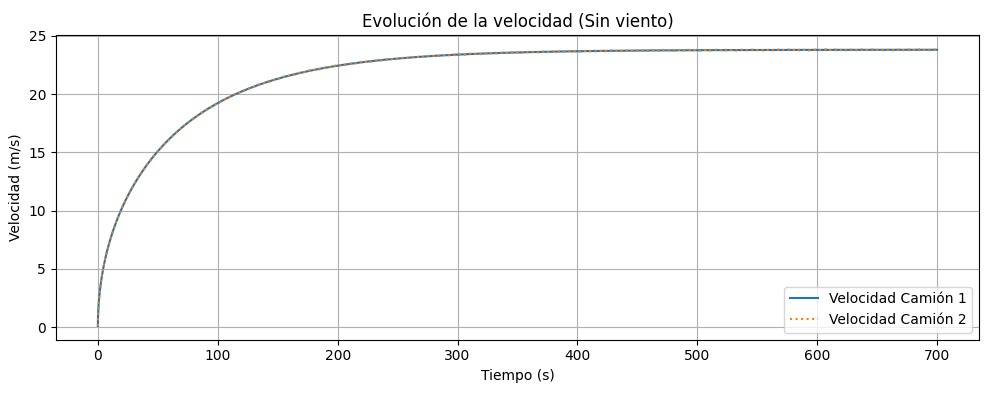
\includegraphics[width=0.75\linewidth]{figures//Cars/vel 2 trucks si si .png}
    \caption{Velocidad de los camiones}
    \label{fig:enter-label}
\end{figure}

La velocidad aumenta de manera exponencial al principio, lo que sugiere una aceleración inicial fuerte, esto debido a la fuerza propulsiva aplicada a cada camión. 

Después de aproximadamente 500 segundos, la velocidad se estabiliza alrededor de 25 m/s (Velocidad máxima permitida en Carreteras) para los tres camiones, con pequeñas fluctuaciones las cuales indican que los camiones ajustan su velocidad para mantener una separación constante.

Las líneas de los tres camiones se superponen casi perfectamente, lo que implica que todos alcanzan la misma velocidad de crucero y se mueven de manera sincronizada, un comportamiento esperado en un modelo ideal sin perturbaciones externas como el viento.

Luego, se analizan las posiciones de los camiones.

\begin{figure}[H]
    \centering
    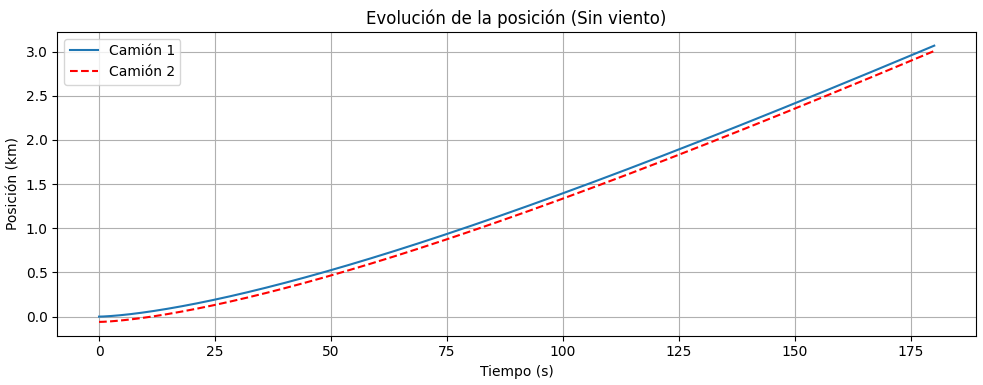
\includegraphics[width=0.75\linewidth]{figures//Cars/evo posi 2 truck.png}
    \caption{Posición entre dos camiones}
    \label{fig:enter-label}
\end{figure}

La posición de los 2 camiones aumenta linealmente con el tiempo después, lo que es consistente con una velocidad constante (como se observó en la gráfica de velocidad).

La pendiente de las líneas es idéntica para los dos camiones, lo que confirma que mantienen la misma velocidad de crucero. Sin embargo, las líneas no se superponen: el Camión 1 está adelante, seguido por el Camión 2 siempre manteniendo la distancia mínima reglamentaria con pequeñas variaciones.

\begin{figure}[H]
    \centering
    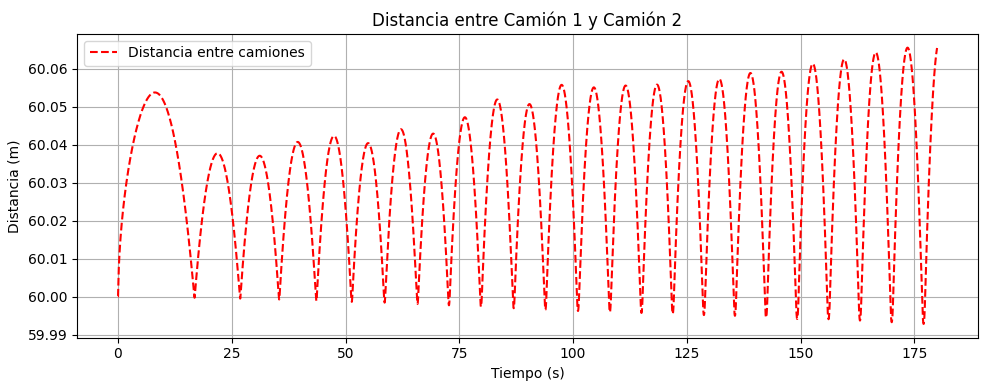
\includegraphics[width=0.75\linewidth]{head way 2 trucks.png}
    \caption{Distancia entre los dos camiones}
    \label{fig:enter-label}
\end{figure}

Se evidencia que la separación entre camiones no varia en gran cantidad manteniendo el headway como se esperaría.

Además, se observa el comportamiento de la potencia y su relación con el consumo de combustible.


\begin{figure}[H]
    \centering
    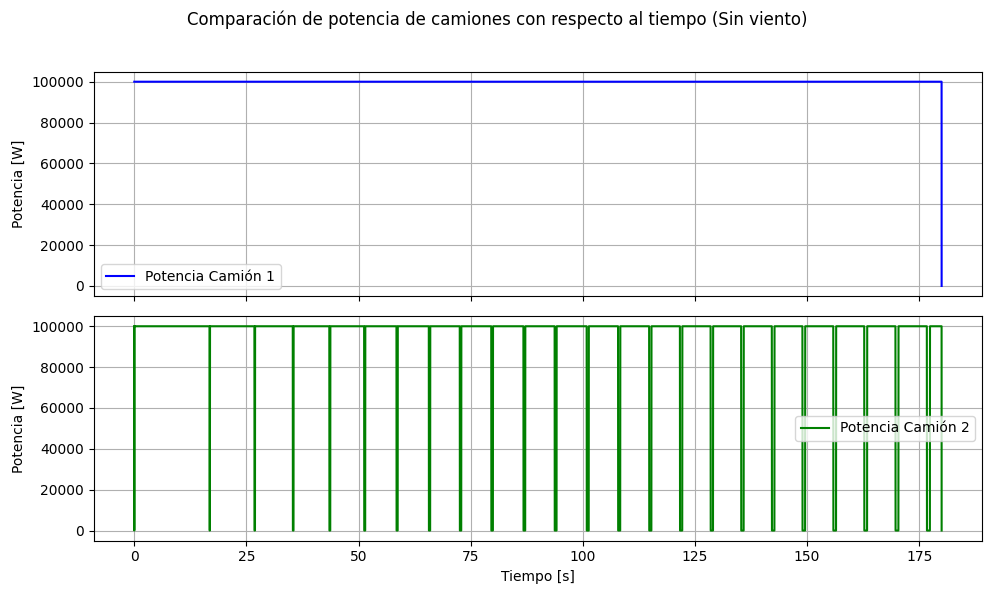
\includegraphics[width=0.75\linewidth]{figures//Cars/Pot 2 trucks .png}
    \caption{Potencia motores}
    \label{fig:enter-label}
\end{figure}

La potencia del camión 1 se mantiene constante puesto que es el líder del pelotón, mientras que la potencia del camión 2 muestra pulsos regulares lo que indica que el camión 2 regula su potencia para mantener la separación ideal con el camión 1. 

\begin{figure}[H]
    \centering
    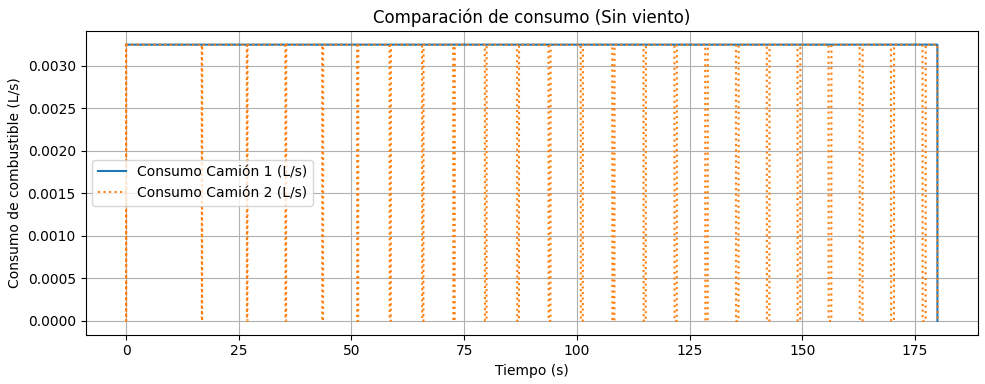
\includegraphics[width=0.75\linewidth]{figures//Cars/comp consu truck 2.png}
    \caption{Relación de Consumo}
    \label{fig:enter-label}
\end{figure}

Con lo visto en la gráfica de potencias, se puede comprender que solo se consume combustible en los momentos donde el camión 2 entrega potencia. Por lo que se puede gráficar el consumo del combustible de los dos camiones

\begin{figure}[H]
    \centering
    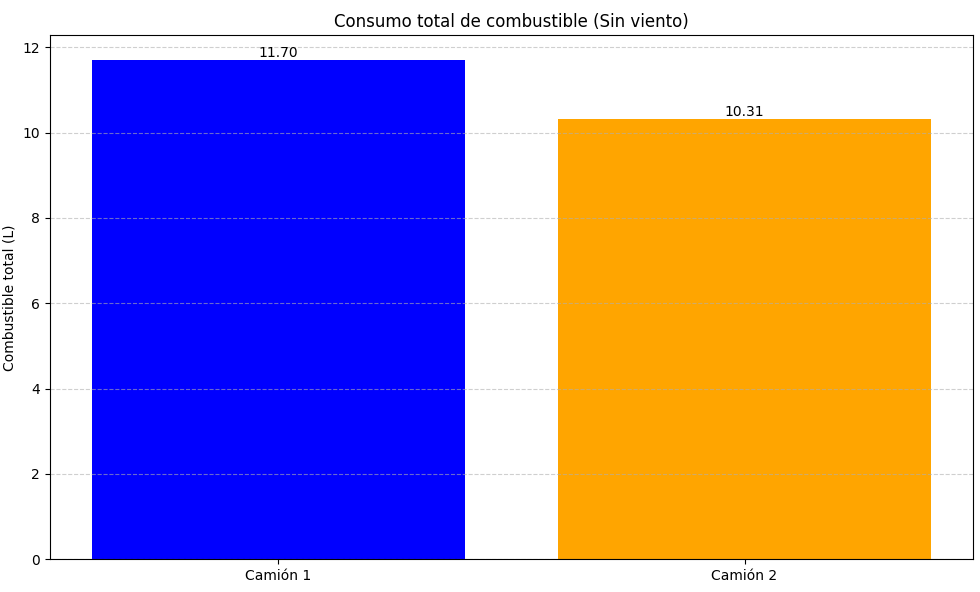
\includegraphics[width=0.55\linewidth]{figures//Cars/Consum combus truck 2.png}
    \caption{Combustible consumido}
    \label{fig:enter-label}
\end{figure}

Se puede observar que el camión 1 consume más combustible puesto a que siempre mantiene la potencia al máximo, mientras que el camión 2, ahorra combustible en los intervalos donde no genera potencia. Realizando así un ahorro de combustible de aproximadamente 13.5\%


\subsubsection{Modelo Refinado - Fuerza del Aire Oscilante}


Las imagenes de este apartado se encuentrane en las del sigueitne iteral en laimagen arriba derecha 


\textbf{Análisis de Resultados Variando Parámetros}


Para analizar la variación de los parámetros, se utilizó el modelo de viento oscilante de tipo sinusoidal, ajustando diferentes variables de entrada. Para las gráficas que se muestran y analizan a continuación, se simularon unicamente $500$ segundos con el fin de poder observar de mejor manera estos resultados.

\begin{enumerate}
    \item \textbf{Variación de Coeficiente de Arrastre.}

    \begin{figure}[H]
        \centering
        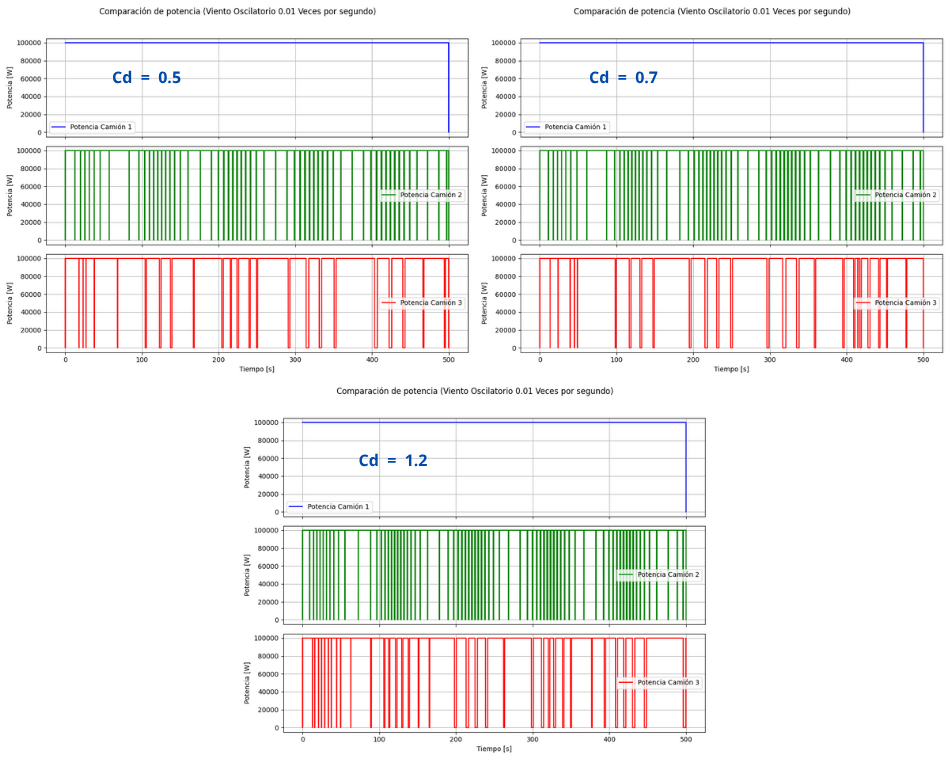
\includegraphics[width=0.8\linewidth]{figures//Cars/cd_variacion.png}
        \caption{Potencia de Camiones por Coeficiente de Arrastre.}
        \label{fig:cd _variation}
    \end{figure}
    
    La gráfica muestra la potencia aplicada por los camiones en función del tiempo para \(C_d = 0.7\) y \(C_d = 0.5\). El camión 1 mantiene una potencia constante de 100 kW, mientras que los camiones 2 y 3 muestran pulsos regulares para mantener la distancia mínima de 60 m. Con \(C_d = 0.5\), los pulsos son menos frecuentes, indicando que una menor resistencia aerodinámica reduce la potencia necesaria, mejorando la eficiencia energética, especialmente para los camiones seguidores, que se benefician del efecto de estela. (\cite{aero})

    
    \begin{figure}[H]
        \centering
        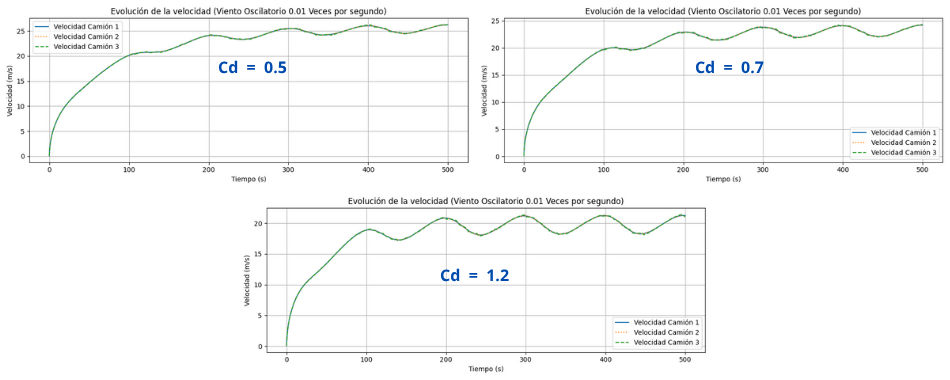
\includegraphics[width=0.75\linewidth]{figures//Cars/vel_cds.png}
        \caption{Perfil Velocidades por Coeficiente de Arrastre.}
        \label{fig:enter-label}
    \end{figure}
    
    La gráfica presenta la velocidad de los camiones, que aumenta rápidamente y oscila cerca de 25 m/s debido al viento sinusoidal (\(v_w(t) = 10.5 \sin(2\pi \cdot 0.01 t)\)). Con \(C_d = 0.5\), las fluctuaciones son menores y la velocidad de crucero se alcanza más rápido que con \(C_d = 0.7\), ya que un menor arrastre estabiliza la dinámica. Los camiones 2 y 3 muestran pequeñas diferencias respecto al camión 1, pero con \(C_d = 0.5\), la sincronización del convoy mejora.

    \begin{figure}[H]
        \centering
        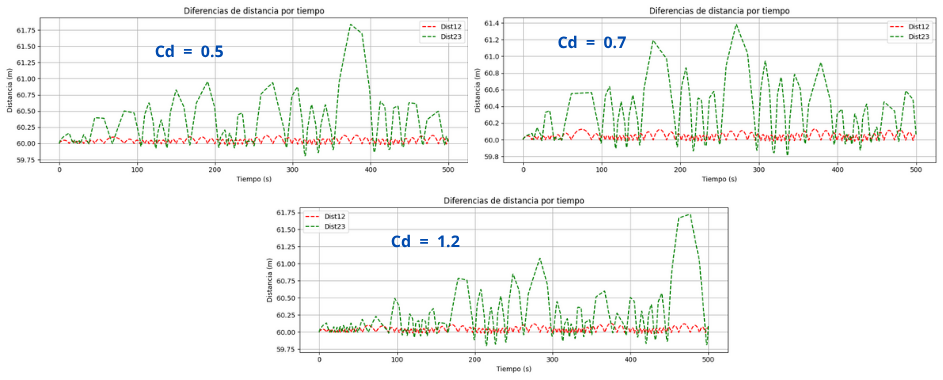
\includegraphics[width=0.75\linewidth]{figures//Cars/headway_cds.png}
        \caption{Separación entre camiones por Coeficiente de Arrastre.}
        \label{fig:enter-label}
    \end{figure}
    La gráfica muestra la distancia entre camiones oscilando alrededor de 60 m, influenciada por el viento sinusoidal. Con \(C_d = 0.5\), las fluctuaciones son menos pronunciadas que con \(C_d = 0.7\), lo que indica que un menor arrastre estabiliza la separación, reduciendo la variabilidad del headway. Esto mejora la seguridad y eficiencia del convoy, minimizando riesgos de colisión y optimizando el efecto de estela.


\item \textbf{Variación Frecuencia del Viento}

\begin{figure}[H]
    \centering
    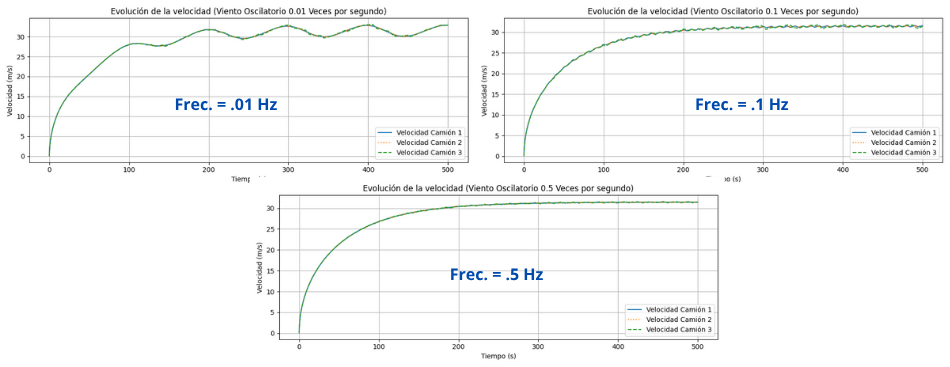
\includegraphics[width=0.75\linewidth]{figures//Cars/vel_hz.png}
    \caption{Perfil de Velocidades por Frecuencia del viento en contra. }
    \label{fig:enter-label}
\end{figure}
    La gráfica muestra las velocidades de los camiones oscilando cerca de 25 m/s, afectadas por el viento sinusoidal. A frecuencias altas (\(\omega = 2\pi \cdot 0.1 \, \text{rad/s}\)), las oscilaciones son rápidas y de baja amplitud, mientras que a frecuencias bajas (\(\omega = 2\pi \cdot 0.01 \, \text{rad/s}\)), son más lentas y amplias. Los camiones 2 y 3 tienen oscilaciones desfasadas, pero a frecuencias altas, el control de potencia responde mejor, estabilizando el convoy.


\begin{figure}[H]
    \centering
    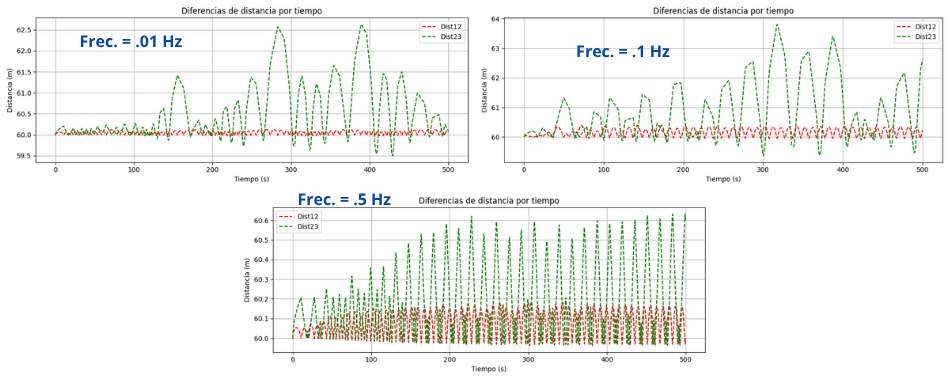
\includegraphics[width=0.75\linewidth]{figures//Cars/dist_hz.png}
    \caption{\textit{Headway} por Frecuencia del viento en contra. }
    \label{fig:enter-label}
\end{figure}
    La gráfica muestra la separación entre camiones oscilando alrededor de 60 m. A frecuencias altas, las fluctuaciones son rápidas y pequeñas, lo que estabiliza el headway. A frecuencias bajas, las oscilaciones son más amplias, aumentando la variabilidad de la distancia y el riesgo de perder el efecto de estela o acercarse demasiado, lo que requiere un control de potencia más robusto para mantener la eficiencia.



\item \textbf{Variación Potencia del Motor}

\begin{figure}[H]
    \centering
    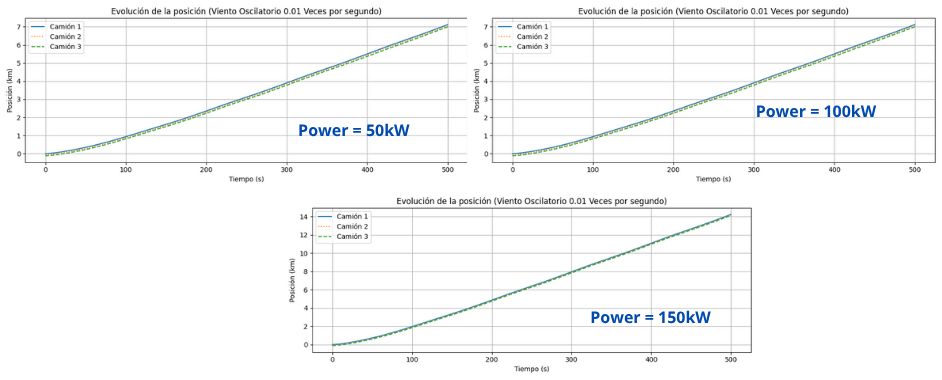
\includegraphics[width=0.75\linewidth]{figures//Cars/pos_power.png}
    \caption{Variación Posición Camiones por Potencia de Motor.}
    \label{fig:enter-label}
\end{figure}
La gráfica muestra la posición de los camiones aumentando linealmente tras la aceleración inicial, con una pendiente mayor para potencias altas (\(P_{\text{nominal}} = 120 \, \text{kW}\)) que para potencias bajas (\(P_{\text{nominal}} = 80 \, \text{kW}\)). Los camiones 2 y 3 mantienen la separación, pero con mayor potencia, las transiciones de potencia son más rápidas, reduciendo la variabilidad del \textit{headway}, aunque esto puede aumentar el consumo de combustible en el camión líder.

\begin{figure}[H]
    \centering
    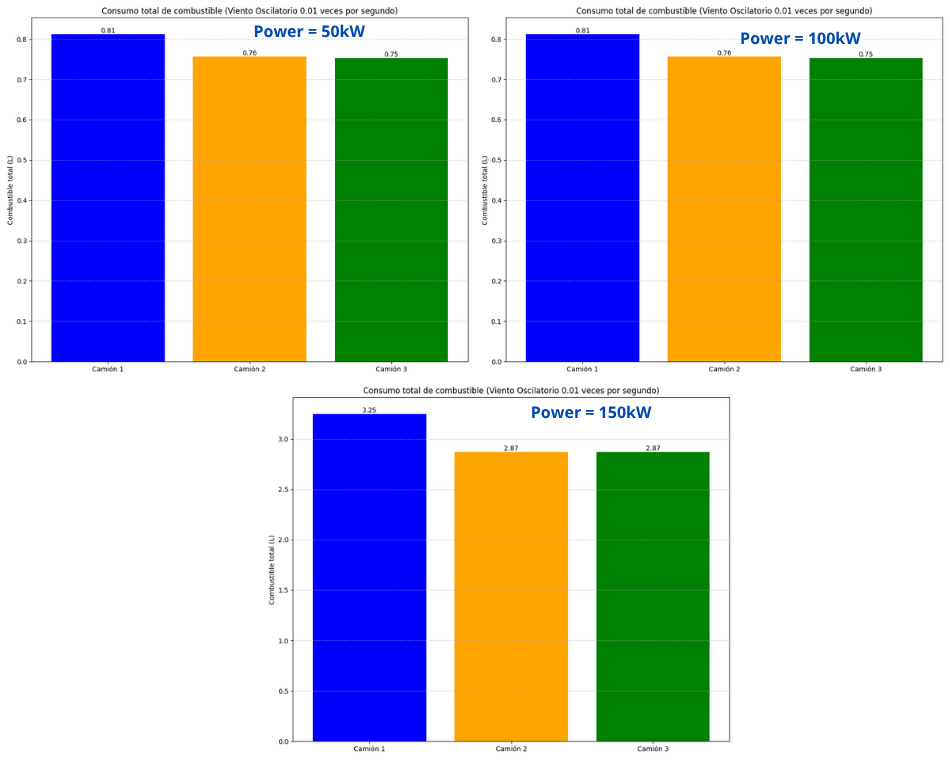
\includegraphics[width=0.75\linewidth]{figures//Cars/gas_power.png}
    \caption{Consumo por Variación de Potencia de Motor.}
    \label{fig:enter-label}
\end{figure}

\textbf{Histograma 1: Consumo total de combustible (POWER = 50 kW)} \\
El consumo es de 0.81 L para Camión 1, 0.76 L para Camión 2 y 0.75 L para Camión 3. El líder (Camión 1) consume más por la mayor resistencia, mientras los seguidores aprovechan el efecto de estela, reduciendo su consumo en un 6-7%.

\textbf{Histograma 2: Consumo total de combustible (POWER = 100 kW)} \\
El consumo permanece en 0.81 L (Camión 1), 0.76 L (Camión 2) y 0.75 L (Camión 3), sin cambios respecto a 50 kW, sugiriendo que la velocidad de crucero y el viento no requieren más energía, manteniendo la ventaja aerodinámica de los seguidores.

\textbf{Histograma 3: Consumo total de combustible (POWER = 150 kW)} \\
El consumo sube a 3.25 L (Camión 1), 2.87 L (Camión 2) y 2.87 L (Camión 3). El aumento significativo en el líder refleja mayor esfuerzo contra el viento, mientras los seguidores reducen su consumo un 11.7 gracias al efecto de estela.
\end{enumerate}


\subsection{Modelo Refinado - Fuerza del Aire Pulsante}



\begin{figure}[H]
    \centering
    \includegraphics[width=0.5\linewidth]{posición pulsante.png}
    \caption{Posición entre camiones - Viento pulsante}
    \label{figposfdasdf}
\end{figure}

La Figura \ref{figposfdasdf} muestra la evolución de la posición de los camiones a lo largo del tiempo bajo la influencia de un viento pulsante. . El camión líder (Camión 1) se mantiene siempre adelante, seguido por los Camiones 2 y 3, respetando la separación inicial de 60 metros. Los pulsos de viento introducen perturbaciones intermitentes, pero la estrategia de control asegura que los camiones mantengan una separación relativamente estable.



\textbf{Análisis de Resultados Variando Parámetros}


Para analizar la variación de los parámetros, se utilizó el modelo de viento pulsante, ajustando diferentes variables de entrada. Para las gráficas que se muestran y analizan a continuación, se simularon unicamente $500$ segundos con el fin de poder observar de mejor manera estos resultados.

\begin{enumerate}
    \item \textbf{Variación de Coeficiente de Arrastre.}

    \begin{figure}[H]
    \centering
    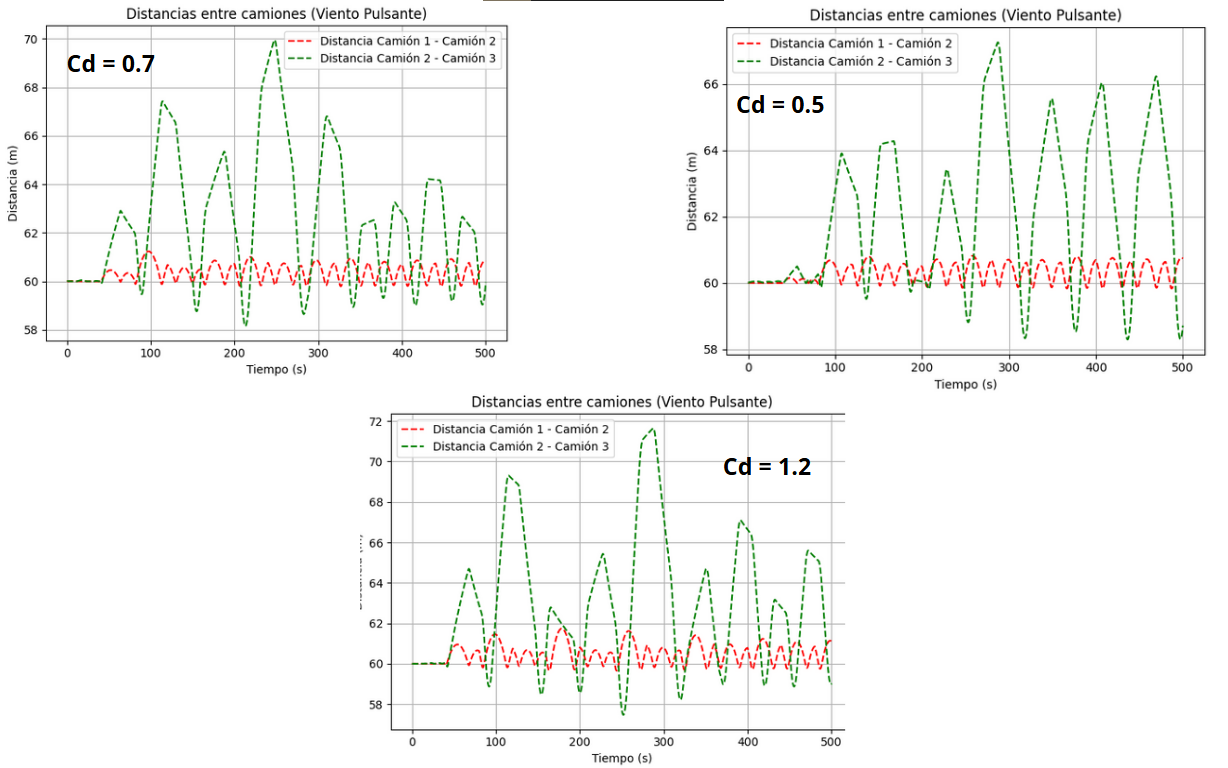
\includegraphics[width=0.75\linewidth]{figures//Cars/posicion cambio cd pulsante.png}
    \caption{Headway por Cd}
    \label{fig:headway_cd}
\end{figure}

La Figura~\ref{fig:headway_cd} representa el \textit{headway} entre camiones consecutivos en función del tiempo, bajo la influencia de un viento pulsante, para diferentes coeficientes de arrastre: $C_d = 0.5$, $C_d = 0.7$ y $C_d = 1.2$. En todos los casos, el \textit{headway} oscila alrededor del valor objetivo de 60 metros.

Con $C_d = 0.5$, las oscilaciones son menores, lo que indica una mayor estabilidad del convoy gracias a una menor resistencia al viento. En cambio, con $C_d = 0.7$, las fluctuaciones aumentan, reflejando mayor sensibilidad a las perturbaciones. Para $C_d = 1.2$, las oscilaciones son aún más amplias, lo que compromete la estabilidad.

Estos resultados muestran que un $C_d$ bajo mejora el control del \textit{headway} y la eficiencia aerodinámica, mientras que un $C_d$ alto incrementa la inestabilidad.


\begin{figure}[H]
    \centering
    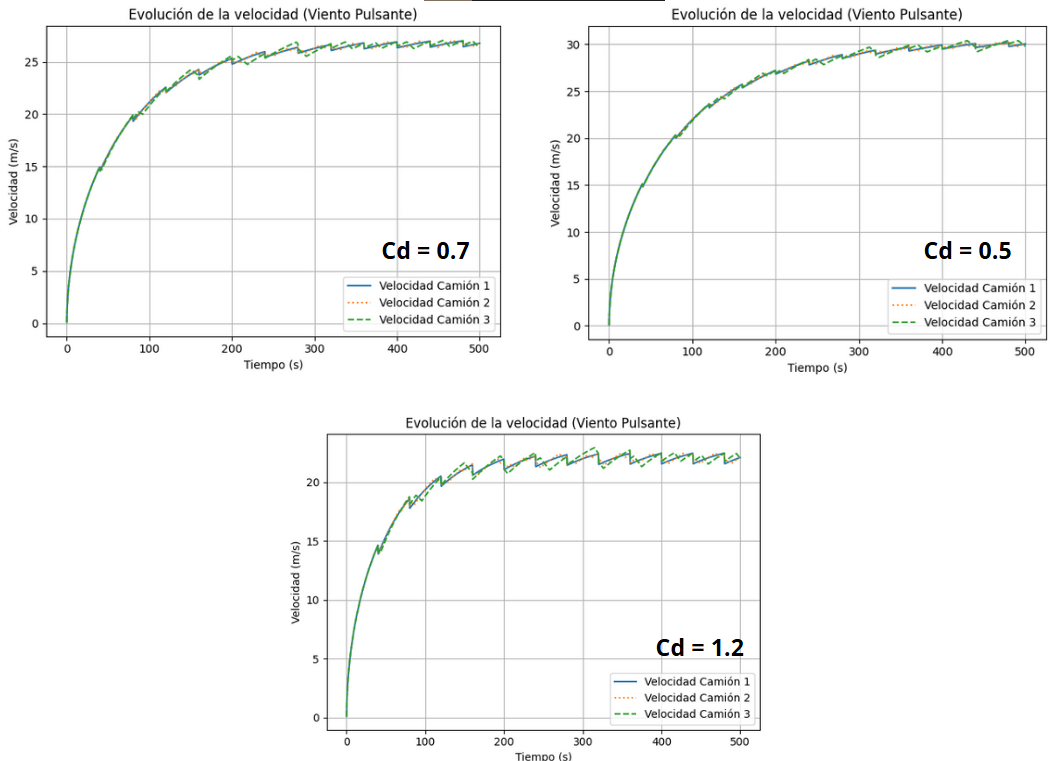
\includegraphics[width=0.75\linewidth]{figures//Cars/var vel punz cd.png}
    \caption{Velocidades por Coeficiente de Arrastre}
    \label{fig:enter-label}
\end{figure}
Muestra los perfiles de velocidad de los camiones a lo largo del tiempo para diferentes coeficientes de arrastre. Las velocidades se estabilizan alrededor de 25 $m/s $ con oscilaciones causadas por el viento pulsante. Para $C_d = 0.7$, las fluctuaciones de velocidad son más marcadas, reflejando una mayor resistencia aerodinámica que amplifica el efecto de los pulsos de viento. Con $C_d = 0.5$, las oscilaciones se atenúan, y los camiones alcanzan la velocidad de crucero más rápidamente y con mayor estabilidad.


\begin{figure}[H]
    \centering
    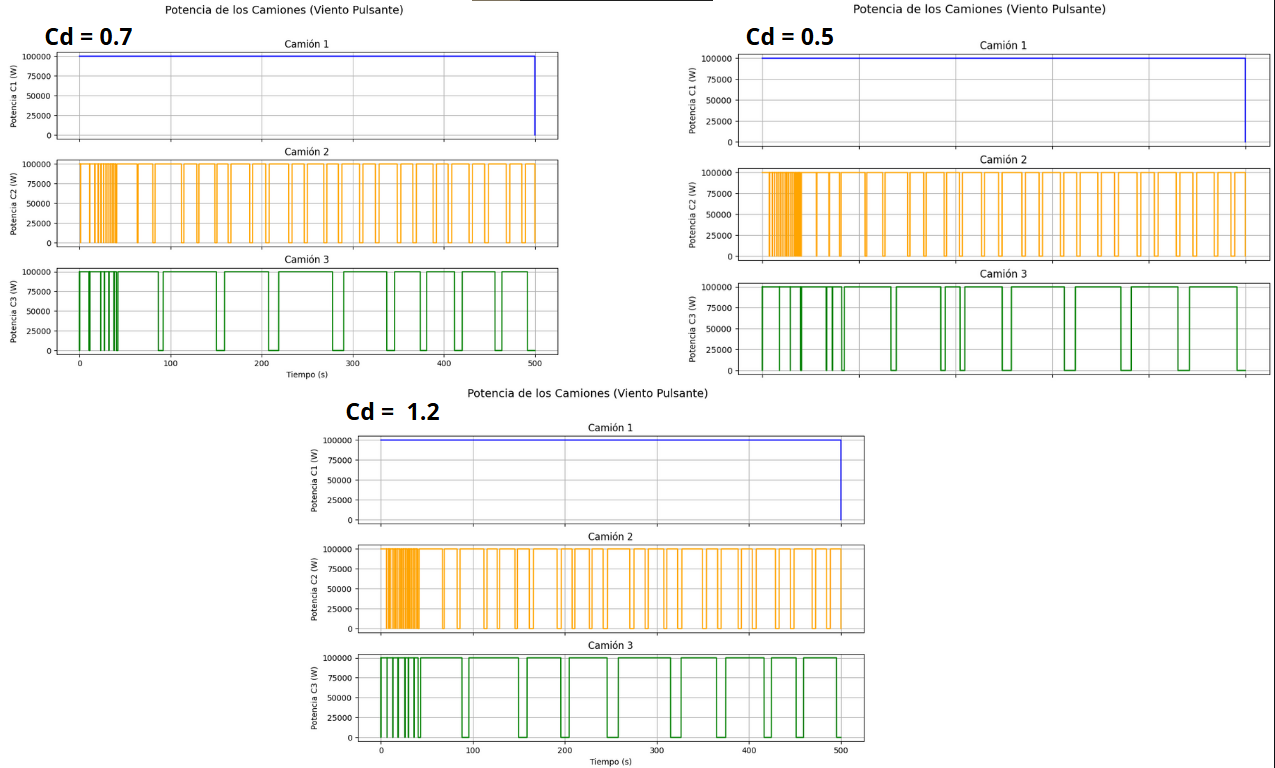
\includegraphics[width=0.75\linewidth]{figures//Cars/pot puls cd.png}
    \caption{Potencia de Camiones por Coeficientes de Arrastre}
    \label{fig:enter-label}
\end{figure}
La potencia aplicada por cada camión a lo largo del tiempo para $C_d = 0.7$ y $C_d = 0.5$. El Camión 1 mantiene una potencia constante de 100 kW, ya que es el vehículo líder y no se beneficia del efecto de estela. Los Camiones 2 y 3 presentan una aplicación de potencia pulsante, ajustándola para mantener el headway mínimo de 60 metros. Con $C_d = 0.7$, los pulsos de potencia son más frecuentes e intensos, ya que el mayor arrastre requiere ajustes más constantes para contrarrestar las perturbaciones del viento. Para $C_d = 0.5$, los pulsos son menos frecuentes y de menor magnitud, lo que indica que la reducción del arrastre disminuye la potencia necesaria para mantener la separación y velocidad deseadas. Esto resulta en una mayor eficiencia energética, especialmente para los camiones seguidores, que se benefician de la menor resistencia aerodinámica debido al efecto de estela.




\item \textbf{Variación Amplitud del Viento}

\begin{figure}[H]
    \centering
    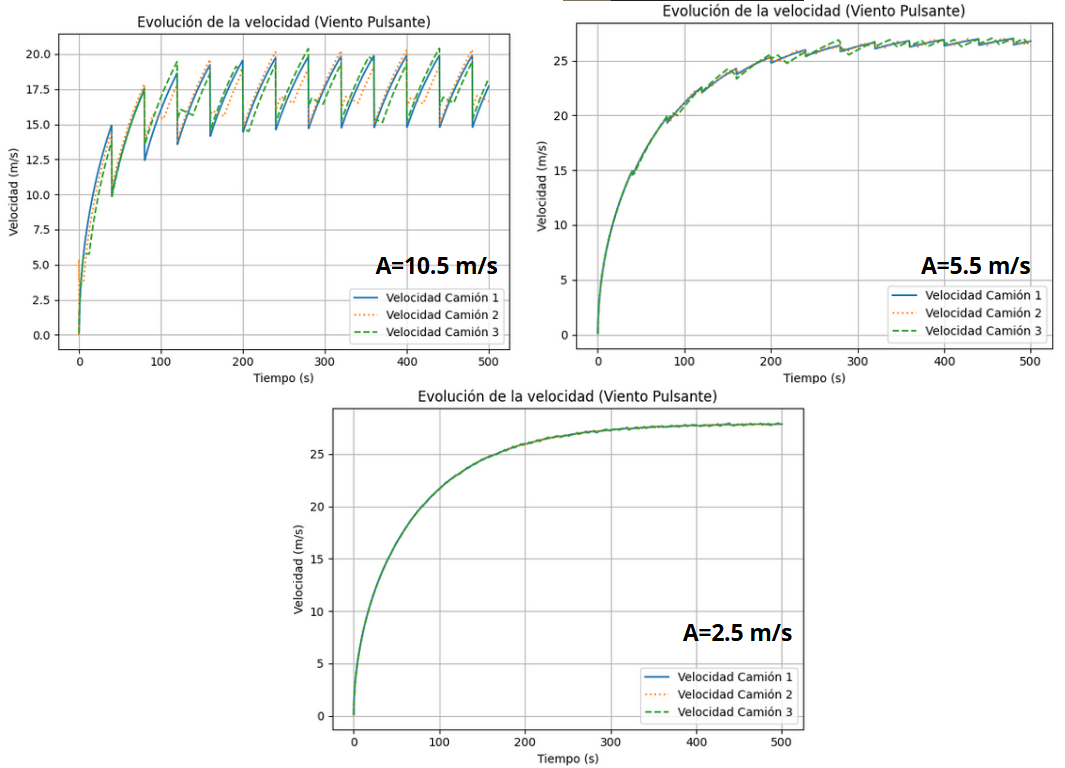
\includegraphics[width=0.75\linewidth]{figures//Cars/vel pul ampl xd.png}
    \caption{Velocidades por Amplitud del Aire}
    \label{fig:enter-label}
\end{figure}

\begin{figure}[H]
    \centering
    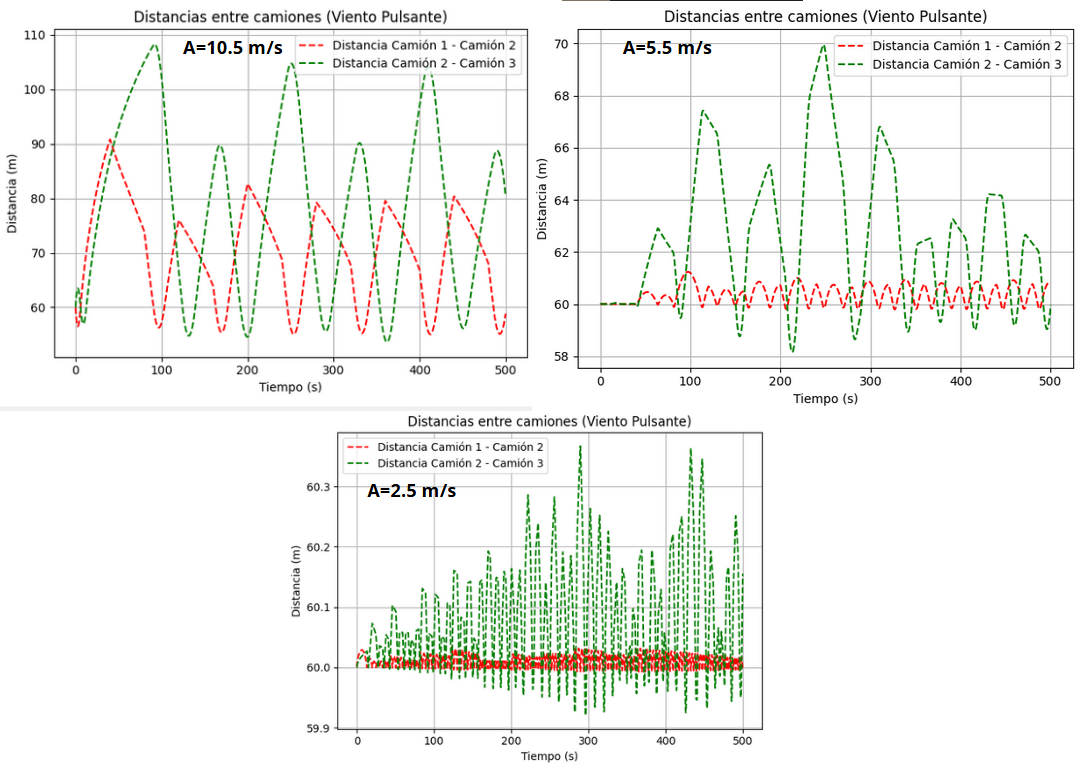
\includegraphics[width=0.75\linewidth]{figures//Cars/head pul ampl xd.png}
    \caption{Headway por Amplitud del Viento}
    \label{fig:enter-label}
\end{figure}

\begin{figure}[H]
    \centering
    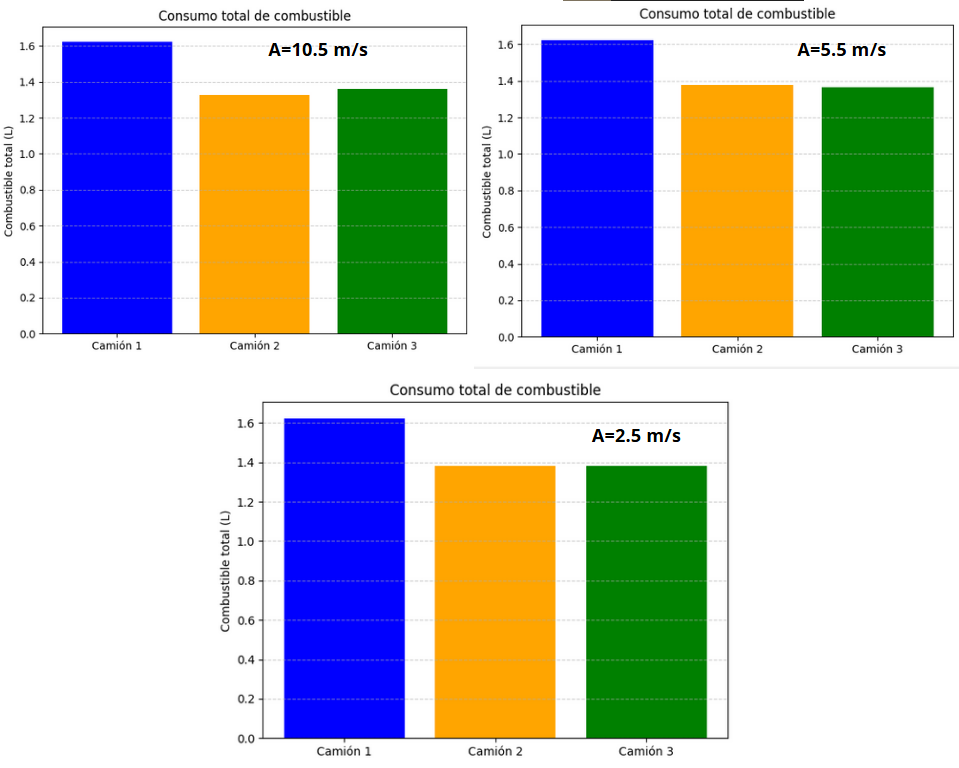
\includegraphics[width=0.75\linewidth]{figures//Cars/comb pul amp xd.png}
    \caption{Consumo por Amplitud del Viento}
    \label{fig:enter-label}
\end{figure}

\begin{figure}[H]
    \centering
    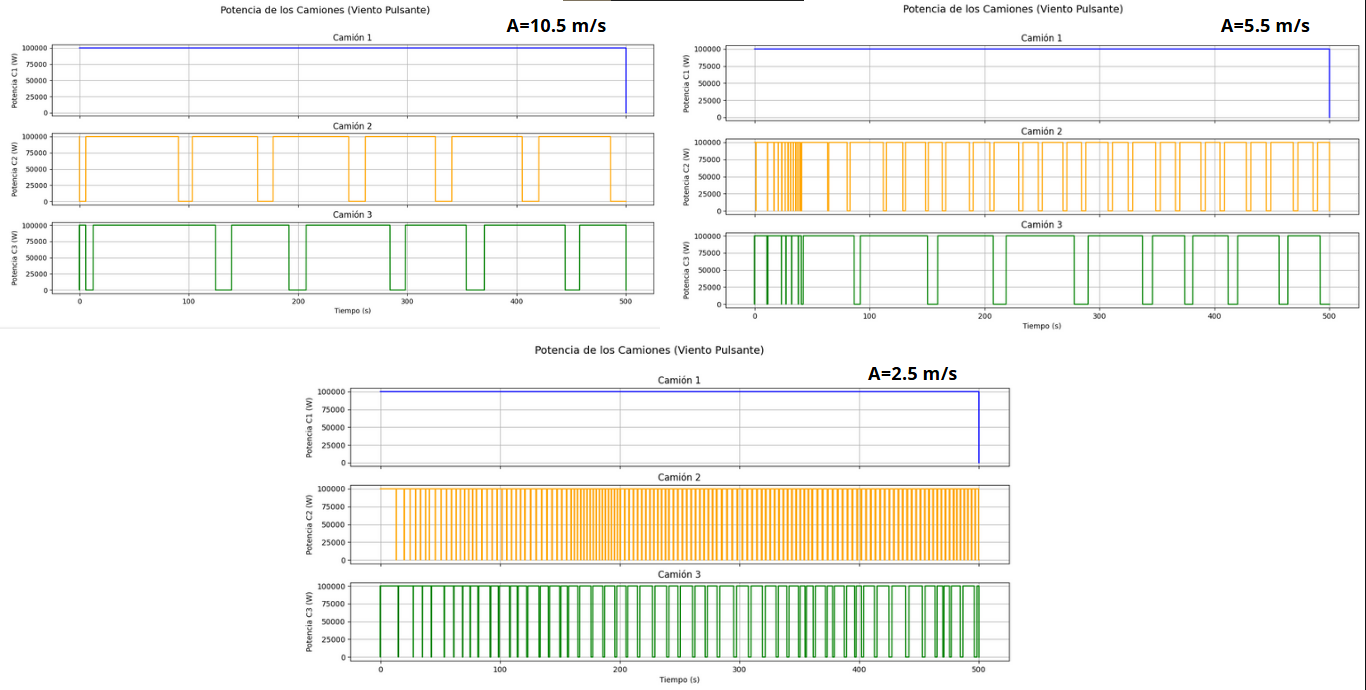
\includegraphics[width=0.75\linewidth]{figures//Cars/pot mot puls ampl xd.png}
    \caption{Potencia por Amplitud del Viento}
    \label{fig:enter-label}
\end{figure}


\end{enumerate}


\subsection{Diseño sugerido}

La resistencia aerodinámica es una fuerza que se opone al movimiento del camión y aumenta con el cuadrado de la velocidad. Esta resistencia está directamente relacionada con el coeficiente de arrastre, el cual depende de la forma del vehículo y su capacidad para cortar el aire eficientemente. Las regiones dominantes de arrastre en un tractor-remolque son la cara frontal del tractor, el
espacio entre el tractor y el remolque, la parte trasera y la base del remolque de modo que en ellas se
presentan las principales pérdidas de energía, consideradas como regiones críticas.(\cite{Aeroreduct})

Se propone una solución en la cual se implementan diferentes piezas aerodinámicas en el camión con el fin de reducir el \(C_d\) de 0.7 a 0.5 (\cite{Aeroreduct}). Las piezas favorecen el flujo del aire a lo largo del camión haciendo.

\begin{itemize}
    \item \textbf{Carenados frontales (superior y laterales)}: Suavizan el flujo alrededor de la cabina.
    \item \textbf{Cubiertas laterales inferiores}: Reducen la turbulencia generada bajo el remolque.
    \item \textbf{Difusor trasero}: Optimiza la forma en que el flujo de aire se separa del vehículo.
    \item \textbf{Generadores de vórtices}: Reorganizan el flujo para minimizar turbulencias en la parte superior.
    \item \textbf{Aletas traseras}: Disminuyen la estela de baja presión que se forma detrás del camión.
\end{itemize}

\begin{figure}[H]
    \centering
    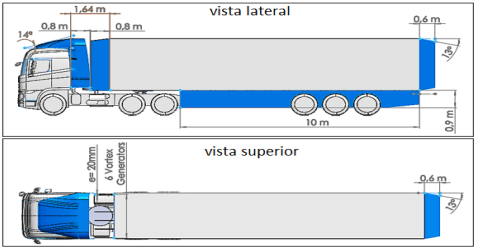
\includegraphics[width=0.55\linewidth]{figures//Cars/Aero truck.png}
    \caption{Vista lateral y superior de un camión con modificaciones aerodinámicas}
    \label{fig:enter-label}
\end{figure}

Según lo mostrado anteriormente, la resistencia del aire es un factor clave que se busca reducir para mejorar la eficiencia de los camiones por si solos, y en general del convoy.

Por lo que la incorporación de mejoras aerodinámicas tiene múltiples beneficios:

\begin{itemize}
    \item Permite \textbf{reducir el headway} sin comprometer la seguridad, gracias a la disminución de turbulencias traseras.

    \begin{figure}[H]
        \centering
        \includegraphics[width=0.65\linewidth]{figures//Cars/distance_differences07.png}
        \caption{Headway con Cd de 0.7}
        \label{fig:enter-label}
    \end{figure}

    \begin{figure}[H]
        \centering
        \includegraphics[width=0.65\linewidth]{figures//Cars/distance_differences cd0.5.png}
        \caption{Headway con Cd de 0.5}
        \label{fig:enter-label}
    \end{figure}

    Como se puede observar, al comparar las imágenes se logra establecer que la variación del headway es menor al tener un \(C_d\) menor.

    
    \item Disminuye la \textbf{fuerza propulsiva necesaria} en cada vehículo, aumentando la eficiencia energética del convoy.

    \begin{figure}[H]
        \centering
        \includegraphics[width=0.45\linewidth]{figures//Cars/total_fuel_consumption 0.7.png}
        \caption{Consumo de Combustible con Cd de 0.7}
        \label{fig:enter-label}
    \end{figure}

    \begin{figure}[H]
        \centering
        \includegraphics[width=0.65\linewidth]{figures//Cars/Consumo combustible cd 0.5.png}
        \caption{Consumo de Combustible con Cd de 0.5}
        \label{fig:enter-label}
    \end{figure}

    Como se logra observar, el consumo de combustible se ve beneficiado al tener menos fuerza de arrastre causada por el aire.

    
    \item Mejora la \textbf{estabilidad dinámica} ante perturbaciones externas como viento en contra.
\end{itemize}

\subsection{Conclusiones}

El modelo simplificado, que considera únicamente la resistencia aerodinámica y la fricción de rodadura, resulta adecuado para estimaciones preliminares del comportamiento de la caravana, aunque subestima el impacto de perturbaciones externas como el viento, lo que limita su precisión en condiciones realistas. En contraste, el modelo refinado incorpora efectos de viento oscilante (sinusoidal) y pulsante (gaussiano), lo que permite una descripción más completa de la dinámica de los camiones, capturando mejor las fluctuaciones en velocidad, separación (headway) y consumo de combustible, y reflejando así condiciones más cercanas a la realidad.

En relación al comportamiento de los vehículos con relación al comportamiento del viento se obtuvo que el viento sinusoidal provoca oscilaciones cíclicas en velocidad y headway: a frecuencias altas (0,1 Hz) las fluctuaciones son rápidas pero de baja amplitud, lo que facilita el control, mientras que a frecuencias bajas (0,01 Hz) las oscilaciones son más amplias, aumentando la variabilidad del headway y el riesgo de colisiones o pérdida del efecto de estela; por su parte, el viento pulsante, mediante ráfagas gaussianas, genera perturbaciones intermitentes que afectan principalmente al camión líder y se transmiten indirectamente a los seguidores.

Además, se comprobó el impacto del \(C_d\) debido a que un menor Cd reduce las fluctuaciones en el headway, estabiliza las velocidades y disminuye la potencia requerida, especialmente para los camiones seguidores que se benefician del efecto de estela.

El camión líder opera con potencia constante (100 kW), mientras que los seguidores ajustan la suya según la distancia al vehículo precedente, llegando incluso a apagarla si el headway cae por debajo de 60 m; este control pulsante en los camiones 2 y 3 se traduce en ahorros de combustible de aproximadamente un 6–13,5 \% respecto al líder, gracias al efecto de estela y la menor potencia requerida. Al aumentar la potencia nominal de los seguidores (de 50 kW a 150 kW), se eleva el consumo de combustible, pero a cambio mejora la respuesta dinámica del convoy y se reduce la variabilidad del headway.



\section{Anexo: Códigos}
En el siguiente \href{https://github.com/Ichibin/Taller01MathModeling}{repositorio} se encuentra la coleccion de los codigos empleados para esta modelacion. Instrucciones en el como ejecutarlos se encuentra en el \texttt{ReadMe} del repositorio.


\printbibliography[heading=secbib]

\end{document}          
